\documentclass{article}
\usepackage{amsmath}
\usepackage{geometry,float}
\usepackage{graphicx}
\usepackage{listings}
\usepackage{color,xcolor}
\usepackage{tcolorbox}
\usepackage{setspace}
\usepackage{subfigure}
\usepackage{longtable}
\tcbuselibrary{skins, breakable, theorems}
\geometry{left=2.3cm,right=2.3cm,top=2cm,bottom=2cm}
\setlength\parindent{20pt} % Removes all indentation from paragraphs

\renewcommand{\labelenumi}{\alph{enumi}.} % Make numbering in the enumerate environment by letter rather than number (e.g. section 6)
%\renewcommand{\baselinestretch}{1.25}
%\usepackage{times} % Uncomment to use the Times New Roman font
\begin{document}
	\newgeometry{top=2.0cm, bottom=2cm}
	\title{Lab 3 Web Development \\ EE 101} 
	\author{\Large{\textbf{https://acemap.lifanz.cn/}}\\ \\Lifan Zhang\\Jiahong Li\\Kaipeng Zeng\\Yanming Liu} 
	\date{2019.5.15} 
	\maketitle 
	\tableofcontents
	\newpage
	\hspace*{0.5cm}
	The aim of our project \emph{PaperHub} is to show the visitors the data about the papers, authors, affiliations and
	other academic units, so as the basis of the project, we need to do some data processing first. First we want to score
	the authors according to the citations of his or her papers, and his or her rank of authors in the papers. The maximum 
	number of authers is 57 in the data provided by the teaching assistant of EE101, so we design a function to weight the 
	academic achievement of the author. Then we calculate the score of each author and affiliation, and write it into two
	new tables in our MySQL database.
	
	\begin{figure}[h]
		\begin{center}
			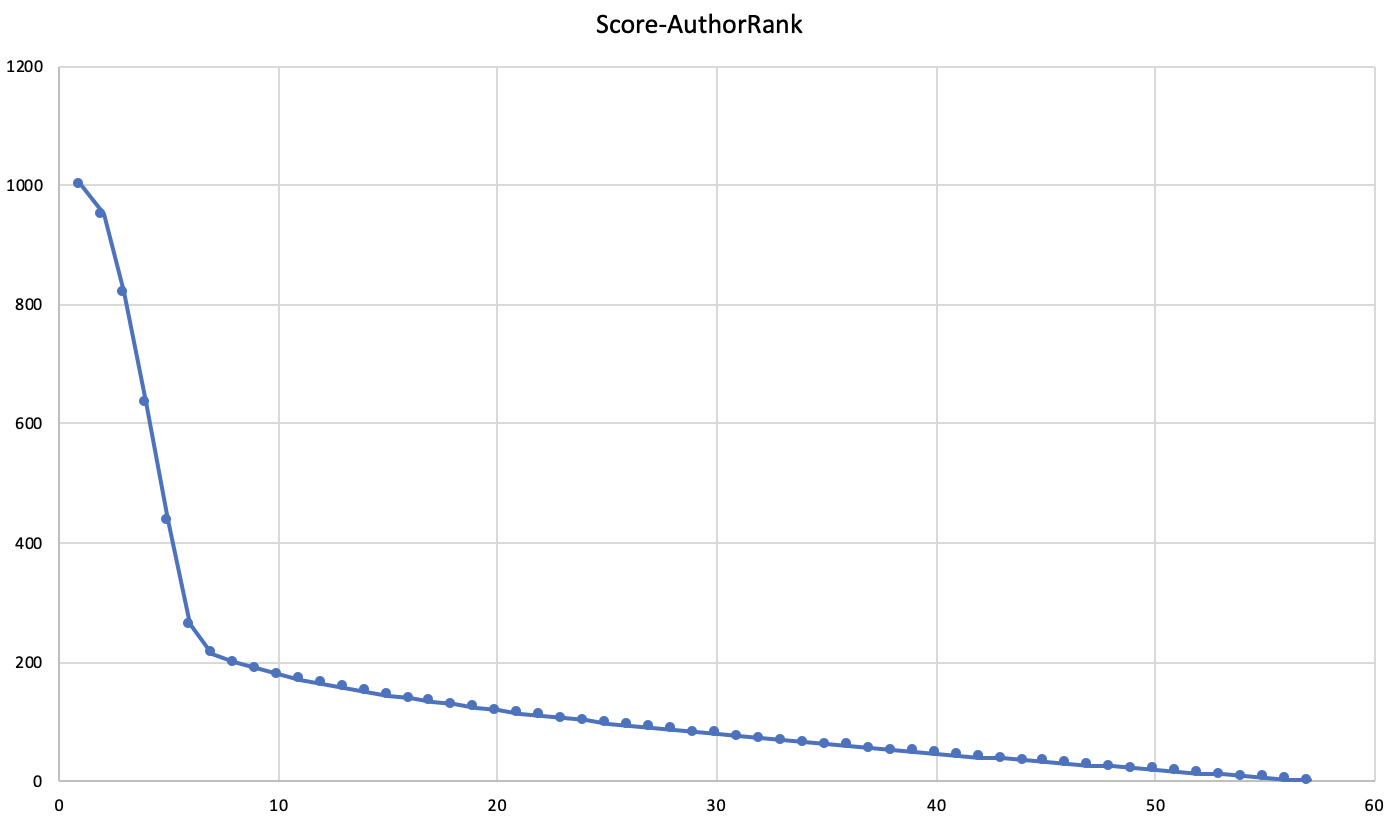
\includegraphics[width=0.95\textwidth]{zlf_1} % Include the image placeholder.png
			\caption{The score range from 2 to 1000}
		\end{center}
	\end{figure}
	
	\section{Website Deployment}
	\hspace*{0.5cm}
	First we buy a domain and an ECS Server from Aliyun and install Ubuntu 18.04. Then we use apt command to install python,
	MySQL, Nginx, PHP and other essential software. After uploading our website to the server through SFTP, we add a server 
	into the configuration of Nginx to let it listen port 80 on the domain acemap.lifanz.cn. To make our website legal, we 
	registered it to MIIT and the public security department, to get an ICP registration number and a public security 
	registration number. Finally, we use certbot the enable SSL connection throught port 443.
	
	\begin{figure}[h]
		\begin{center}
			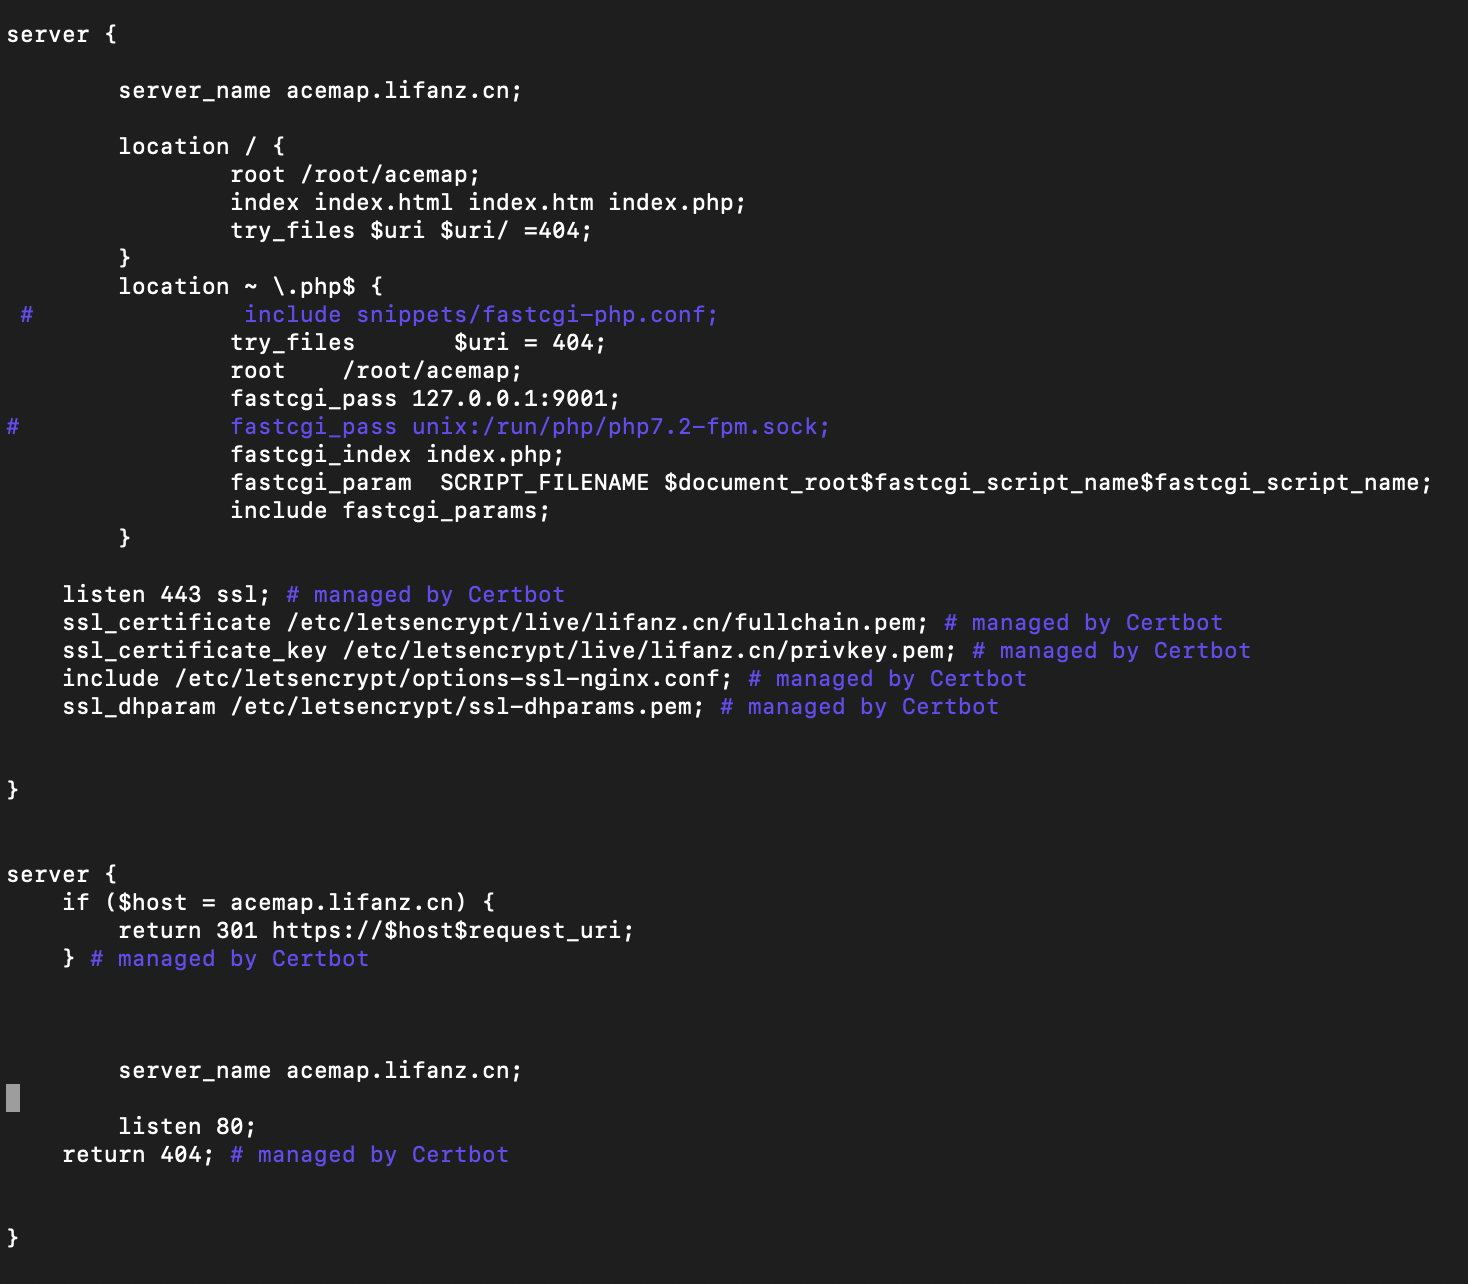
\includegraphics[width=0.90\textwidth]{zlf_2} % Include the image placeholder.png
			\caption{The configuration of Nginx}
		\end{center}
	\end{figure}
	
	\section{Homepage}
	\hspace*{0.5cm}
	In the homepage, we want to realize two functions. The first one is a general searching input box. In the box, the user
	can search everything he want, and the webpage will guess what the user want to search and give the user some hints in a
	dropdown list. The second one is an advanced search form, where the user can specify the type of data he want to get.
	We use bootstrap and a model(https://github.com/BlackrockDigital/startbootstrap) to beautify the homepage.\\
	To realize realtime search suggestion, we built a new solr core, which includes the papers of lots of citations and is much
	smaller than the former one, because if we use the former core, it will take too much time to search. And we need to make
	a search operation when the user press a key on the keyboard, if it is too slow, the experience of the user will be stuck.
	The solr core returns a json array to the homepage, and the homepage will show it in a droplist.
	
	\begin{figure}[H]
		\begin{center}
			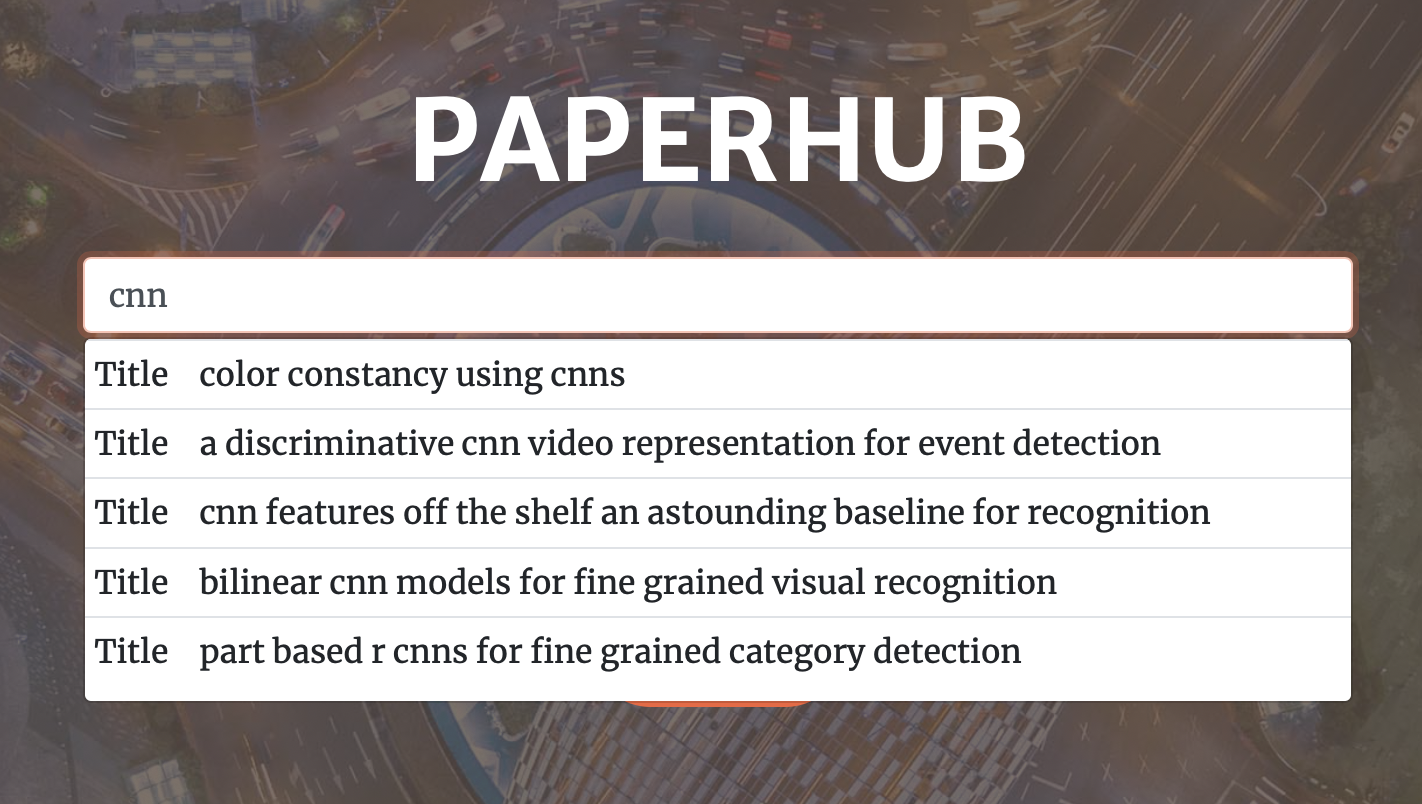
\includegraphics[width=0.80\textwidth]{zlf_3} % Include the image placeholder.png
			\caption{The search suggestion droplist}
		\end{center}
	\end{figure}
	\restoregeometry
	\newgeometry{left=2.3cm,right=2.3cm,top=2cm,bottom=2cm}
	\section{About Search Page}
	\subsection{The Page Layout}
	\begin{figure}[htb]
		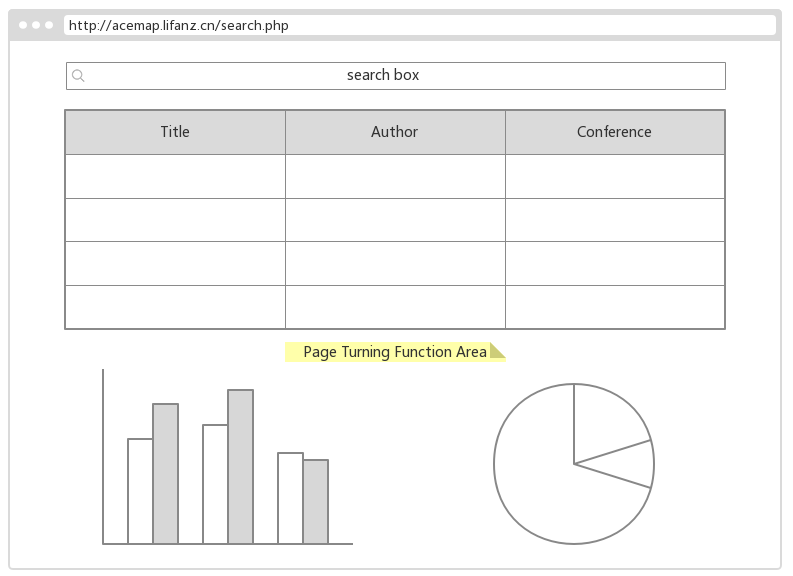
\includegraphics[width=1.0\textwidth]{searchlayout.png}
		\caption{layout}
		\label{searchlayout}
	\end{figure}
	The layout of this page is shown in Figure \ref{searchlayout}. In the top area, we set a search box. In the middle of the page, we use a table to show the search result. And the function area (to turn the page) is just below the table. At the bottom of the page, we show two statistical figures (according to the search result).\\ \\
	\textbf{How to realize this layout?}\\
	Use bootstrap grid layout. Shown in figure \ref{searchlayoutcode}.
	\begin{figure}[htb]
		
\includegraphics[width=0.6\textwidth]{searchlayoutcode1.png}\\
		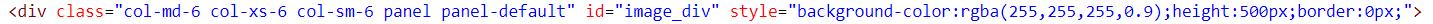
\includegraphics[width=1.0\textwidth]{searchlayoutcode2.png}
		\caption{code}	
		\label{searchlayoutcode}
	\end{figure}
	\subsection{Using Ajax To Realize Interaction}
	\textbf{Why we choose ajax?}\\
	\begin{itemize}
		\item Reload the changing part instead of reloading the whole page $\Rightarrow$  more fluent response
		\item Separate the front-end and the back-end $\Rightarrow$ more clear web design logic
	\end{itemize}
	\textbf{How the ajax work in our search page?}\\
	Shown in figure \ref{ajaxgraph}.
	\begin{figure}[htb]
		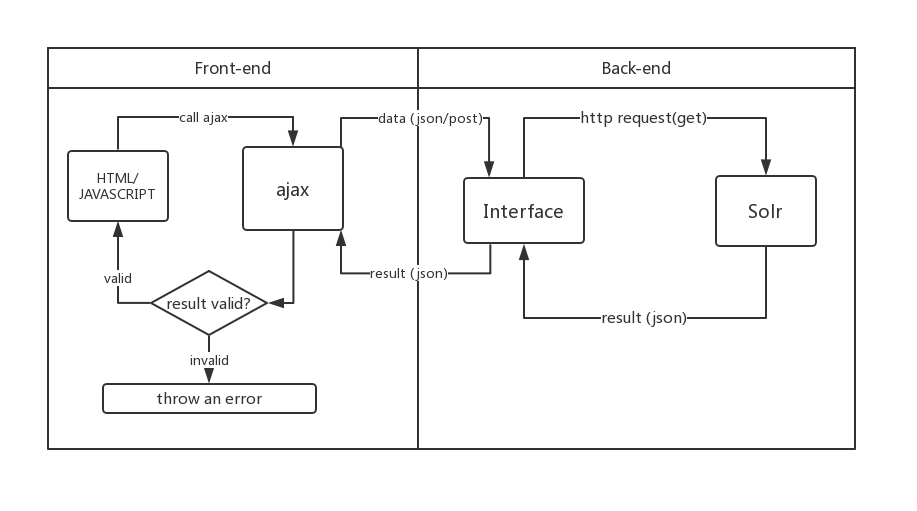
\includegraphics[width=1.0\textwidth]{ajax_graph.png}
		\caption{ajax}
		\label{ajaxgraph}
	\end{figure}\\
	\textbf{How to realize it?}\\
	JQuery.ajax: Just like the code shown in figure \ref{ajaxfigure}\\
	\begin{figure}[htb]
		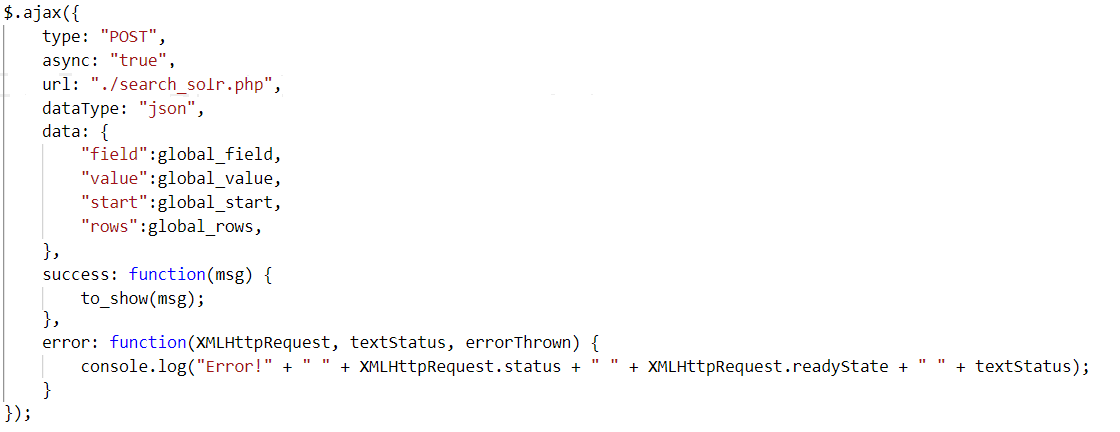
\includegraphics[width=1.0\textwidth]{ajaxfigure.png}
		\caption{ajax code}
		\label{ajaxfigure}
	\end{figure}\\
	Interface: search\_solr.php: Just like the code shown in figure \ref{searchsolr}\\
	\begin{figure}[htb]
		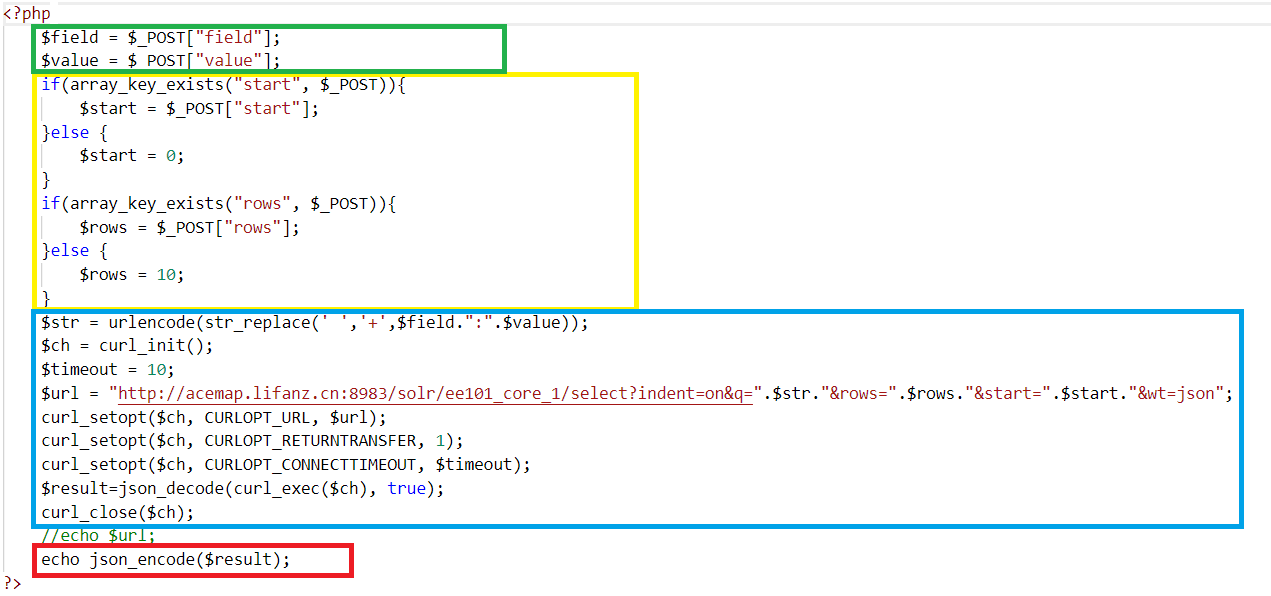
\includegraphics[width=1.0\textwidth]{search_solr_php.png}
		\caption{search\_solr.php code}
		\label{searchsolr}
	\end{figure}\\
	\begin{tabular}{|c|c|}
		\hline
		\textbf{Color}&\textbf{Function}\\
		\hline
		\textcolor[rgb]{0,0.5,0.1}{green}&receive data (by post)\\
		\hline
		\textcolor[rgb]{0.9,0.7,0}{yellow}&set default value\\
		\hline
		\textcolor[rgb]{0,0,0.6}{blue}&search in solr (by http request)\\
		\hline
		\textcolor[rgb]{0.9,0,0}{red}&return the result (in json format)\\
		\hline
	\end{tabular}
	\subsection{Paging}
	\subsubsection{Model 1}
	\textbf{UI Design}
	\begin{figure}[htb]
		\centering
		
\includegraphics[width=0.4\textwidth]{paging-ui.png}
		\caption{paging ui design}\label{paging-ui}
	\end{figure}\\
	Imitate google and baidu (figure \ref{paging-ui}).   Associated code: (figure \ref{paging-code})
	\begin{figure}[!h]
		\centering
		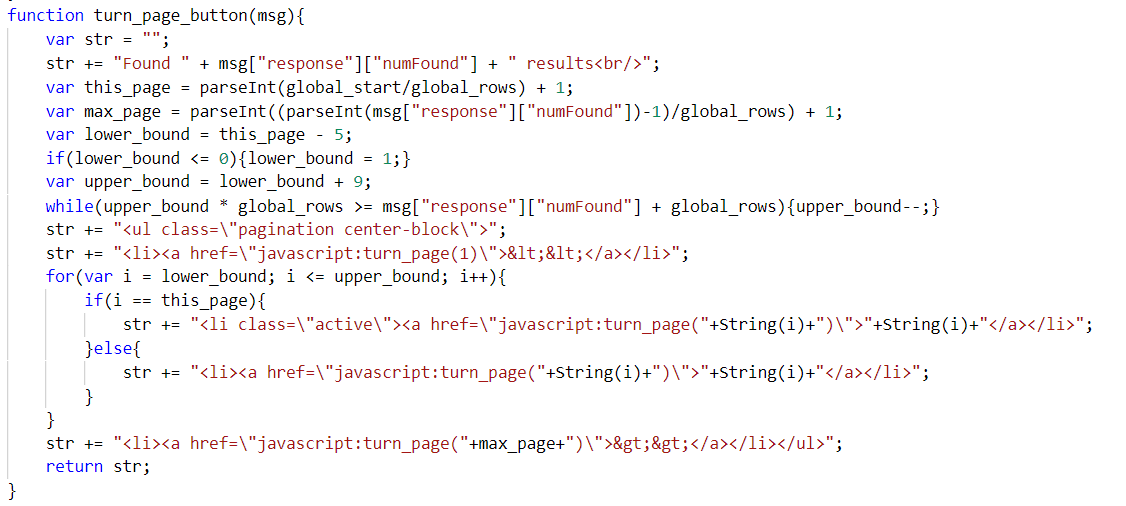
\includegraphics[width=0.65\textwidth]{paging-code.png}
		\caption{paging ui code}\label{paging-code}
	\end{figure}\\
	\textbf{How to realize the paging function?}
	\begin{figure}[htb]
		\centering
		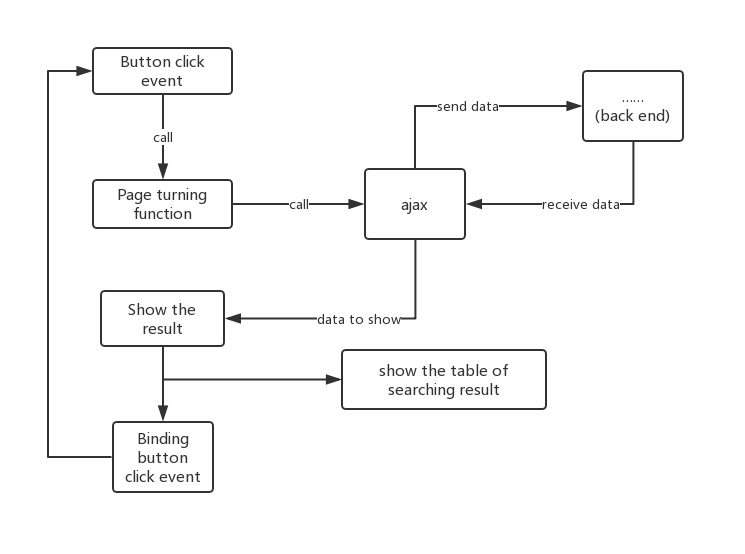
\includegraphics[width=1.0\textwidth]{paging-process.png}
		\caption{page turning}\label{paging-process}
	\end{figure}\\
	\textbf{How to reload the table when turning page?}\\
	We use a simple way: $document.getElementById('div\_id').innerHTML=str;$ where 'str' is a string variable which contains the html codes to show in the new table area. And apparently, the string variable 'str' is produced by the program dynamically according to the search result returned by solr.\\
	
	\noindent \textbf{Model 2}\\
	\indent Move your mouse to the right side of the searching result table and you will see your cursor changing into an arrow, then if you click your mouse, it will turn to the next page. Similarly if you move your mouse to the left side and click it, the web page will turn to the last page.\\
	\indent We realize it in this way: Monitor the mouse moving event. If the cursor is in the detecting area, we change the cursor style in an arrow(left arrow or right arrow) and binding a turning page function to the mouse click event. When your cursor leave this detecting area, we unbind the click event. 
	\subsection{Highlight}
	\begin{longtable}{|p{80pt}|p{340pt}|}
		\hline
		Search box&Set a search box at the top of this page. Users can change the searching words in a more convenient way.\\
		\hline
		Radar map&There are 13 conferences. And the radar map only show the top 6 conferences. So we need to sort them. But after sorting the conferences the shape of the radar map graph will be monotonous. Randomization is the solution.\\
		\hline
		Settings&Using bootstrap popover. Users can click the setting button, then set the number of rows to show, go to a certain page or turn on/off the second paging model.\\
		\hline
		User-friendly reloading&Using ajax to realize paging, there is a problem: when the web page reload, it will go to the first page. But we hope it can remain its original page instead of the first page. To solve this problem, we use session. When the 'onbeforereload' event triggered we write the page records into the session. When 'onload' event triggered we read the records from session.(We have also tried cookie, but session is much better.)\\
		\hline
	\end{longtable}
	\begin{figure}[!h]
		\subfigure{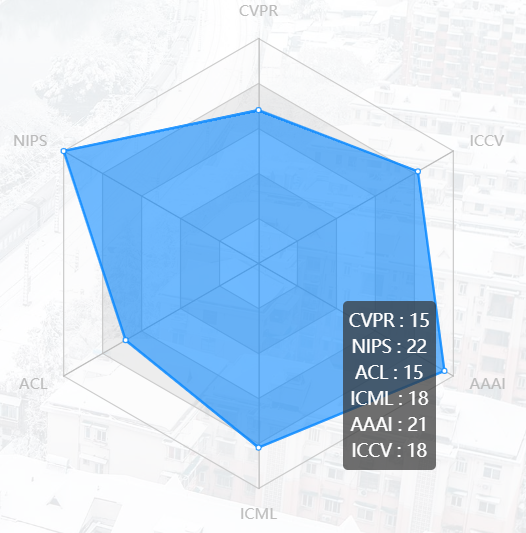
\includegraphics[width=0.5\textwidth]{radar.png}}
		\subfigure{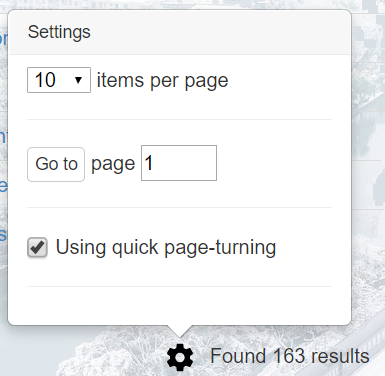
\includegraphics[width=0.5\textwidth]{settings.png}}
	\end{figure}
	\section{About Using Echarts (Author Page And Affiliation Page)}
	\textbf{How can we draw statistical graph using 'Echarts'?}\\
	\begin{itemize}
		\item Know the 'Echarts' API;
		\item Processing and formatting data;
		\item Setting the tooltip;
		\item Adjust the layout.
	\end{itemize}
	
	\noindent\textbf{Know the Echarts' API:}\\
	\indent Such as echarts.init(), echarts.setOption(), echarts.legend, echarts.tooltip, echarts.event. We can get the direction for use in the official API document.\\
	\noindent\textbf{Processing and formatting data:}\\
	\indent After we decide in which type of diagram to show the data we get, we should format the data to make it fit the diagram. Different types of diagram require different data format. We can know the required data format for a certain diagram type in the way shown below(figure \ref{dataformat})
	\begin{figure}[!h]
		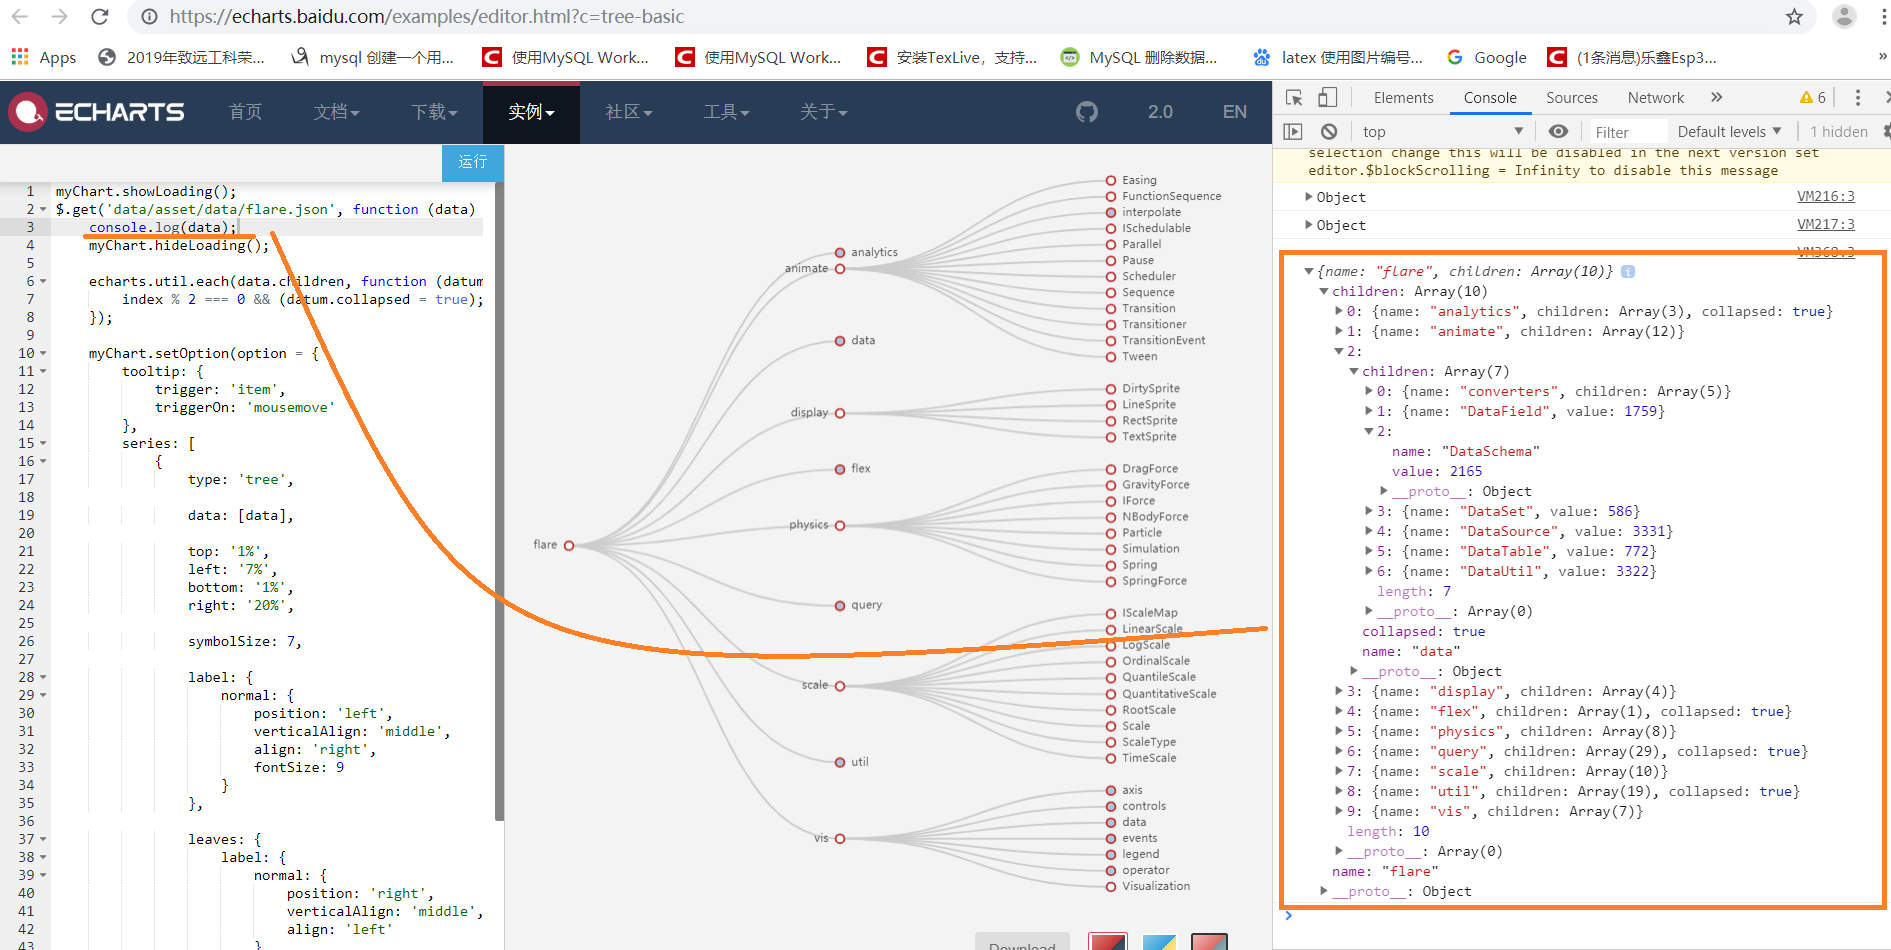
\includegraphics[width=1.0\textwidth]{formatdata.png}
		\caption{Know the required data format}
		\label{dataformat}
	\end{figure}\\
	\indent We write the code `console.log(data);` in the left coding area. And we can find the output in the browser console. And we can see in this case the data is formatted in JSON, and it expresses the tree relationship by recursively nested arrays.\\
	\indent We process the data in a specialized php program. To process a tree graph, I wrote the code below.(figure \ref{Tree graph code})
	\begin{figure}[!h]
		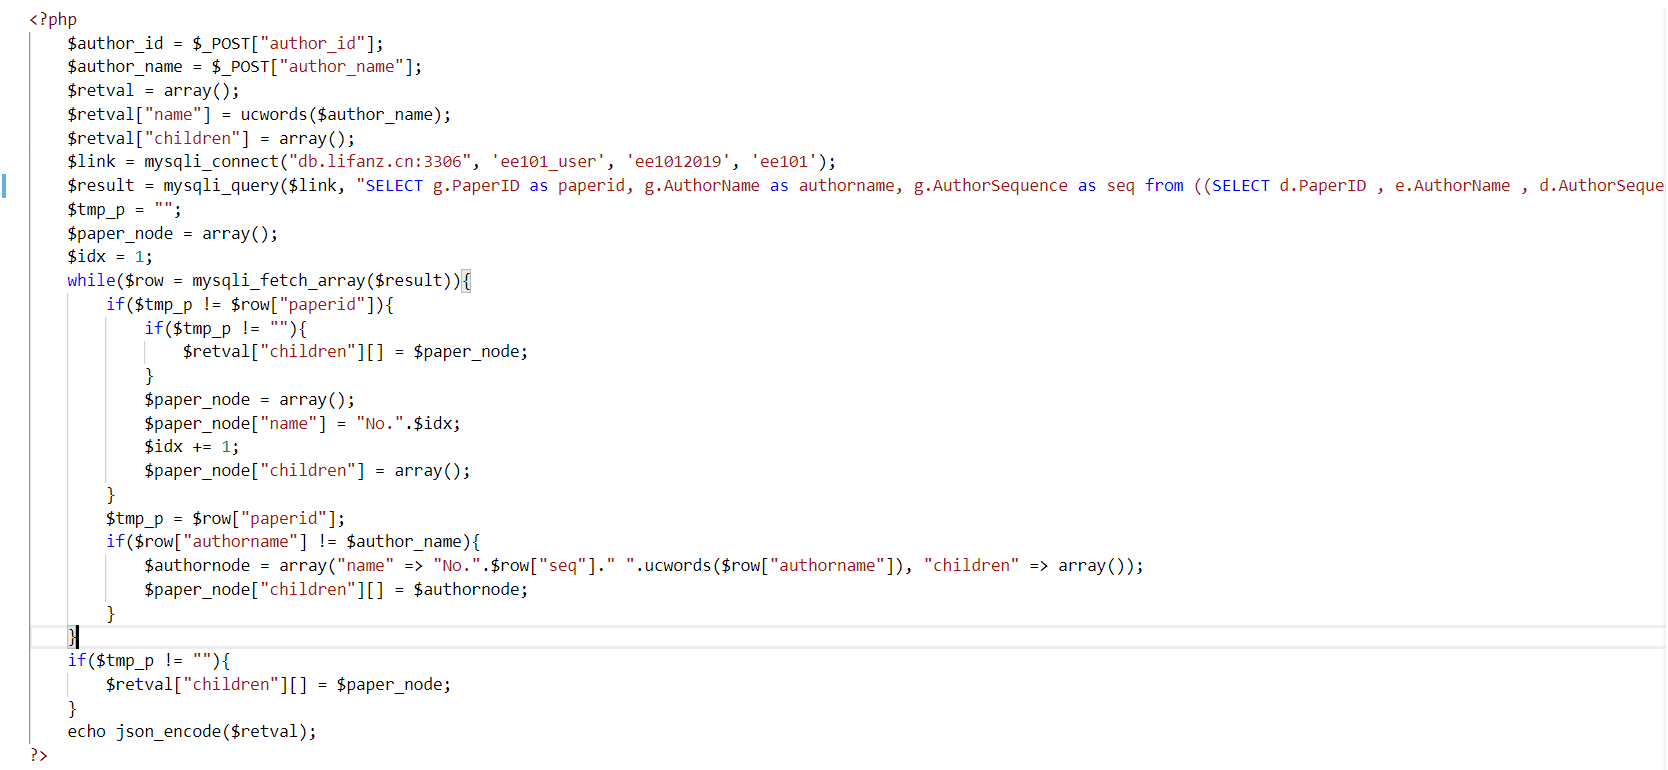
\includegraphics[width=1.0\textwidth]{treegraphcode.png}
		\caption{source code}
		\label{Tree graph code}
	\end{figure}\\
	\indent We search the data in solr or in mySQL, and deal with data by php or javascript, then show the diagram. When the data is relatively simple, it works well. But sometimes the data is too complex to deal with in this way. Maybe the scale of data is too large, or maybe the data is gotten from the relatively complex calculating. In these cases, if we deal with the data  dynamicly, the page will be very slow and not smooth. So for some complex graph (such as 3D bar graph and force oriented author map), we use this method: preprocess the data off-line, but render the graph dynamicly. We preprocess the data by c++ (reading data information from the txt file) and python (getting data information from the mySQL).
	\begin{figure}[!h]
		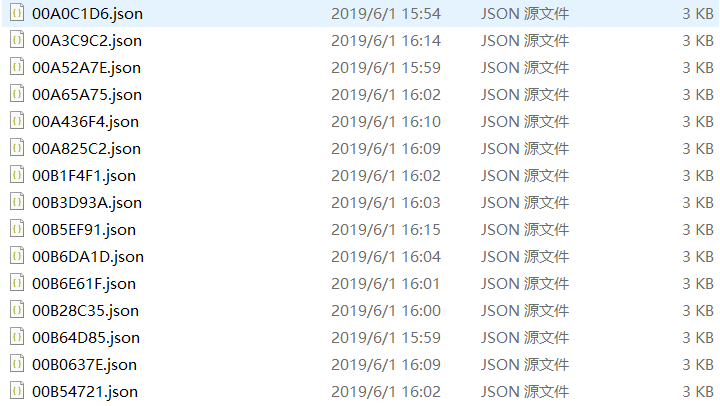
\includegraphics[width=0.5\textwidth]{preprocess.png}
		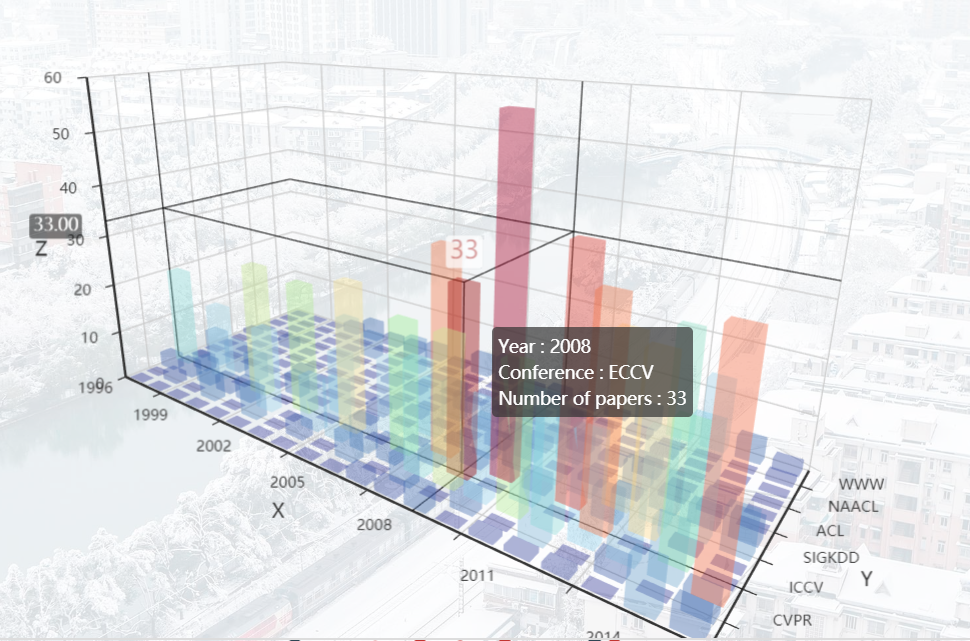
\includegraphics[width=0.5\textwidth]{threeDbar.png}
		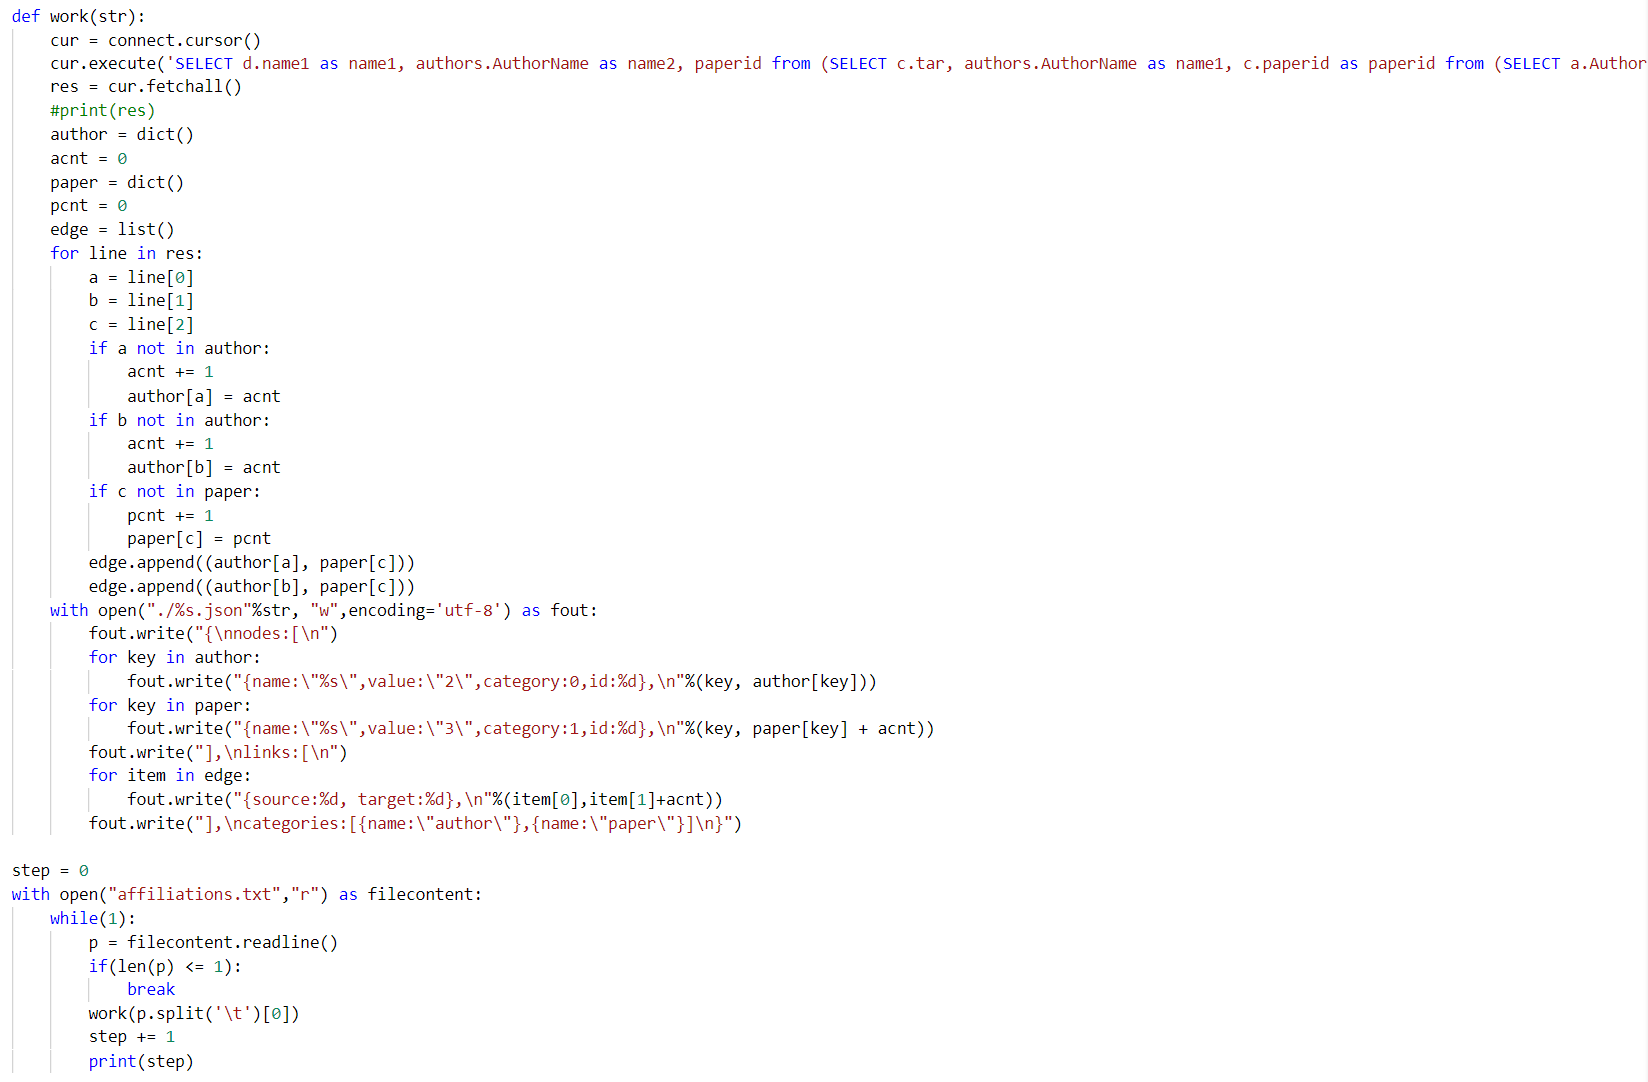
\includegraphics[width=0.5\textwidth]{pythoncode.png}
		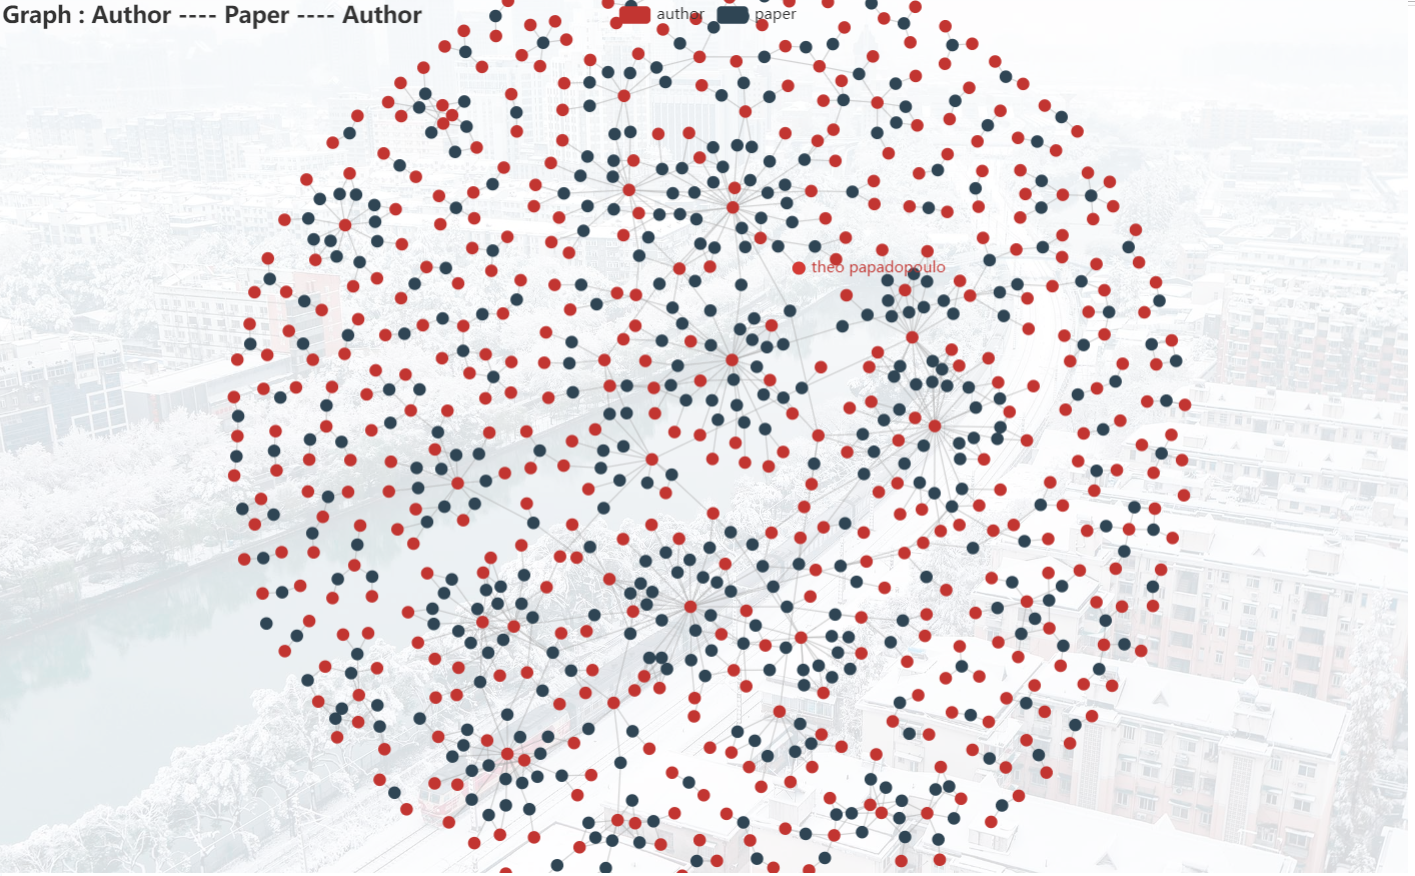
\includegraphics[width=0.5\textwidth]{forceorientedauthormap.png}
		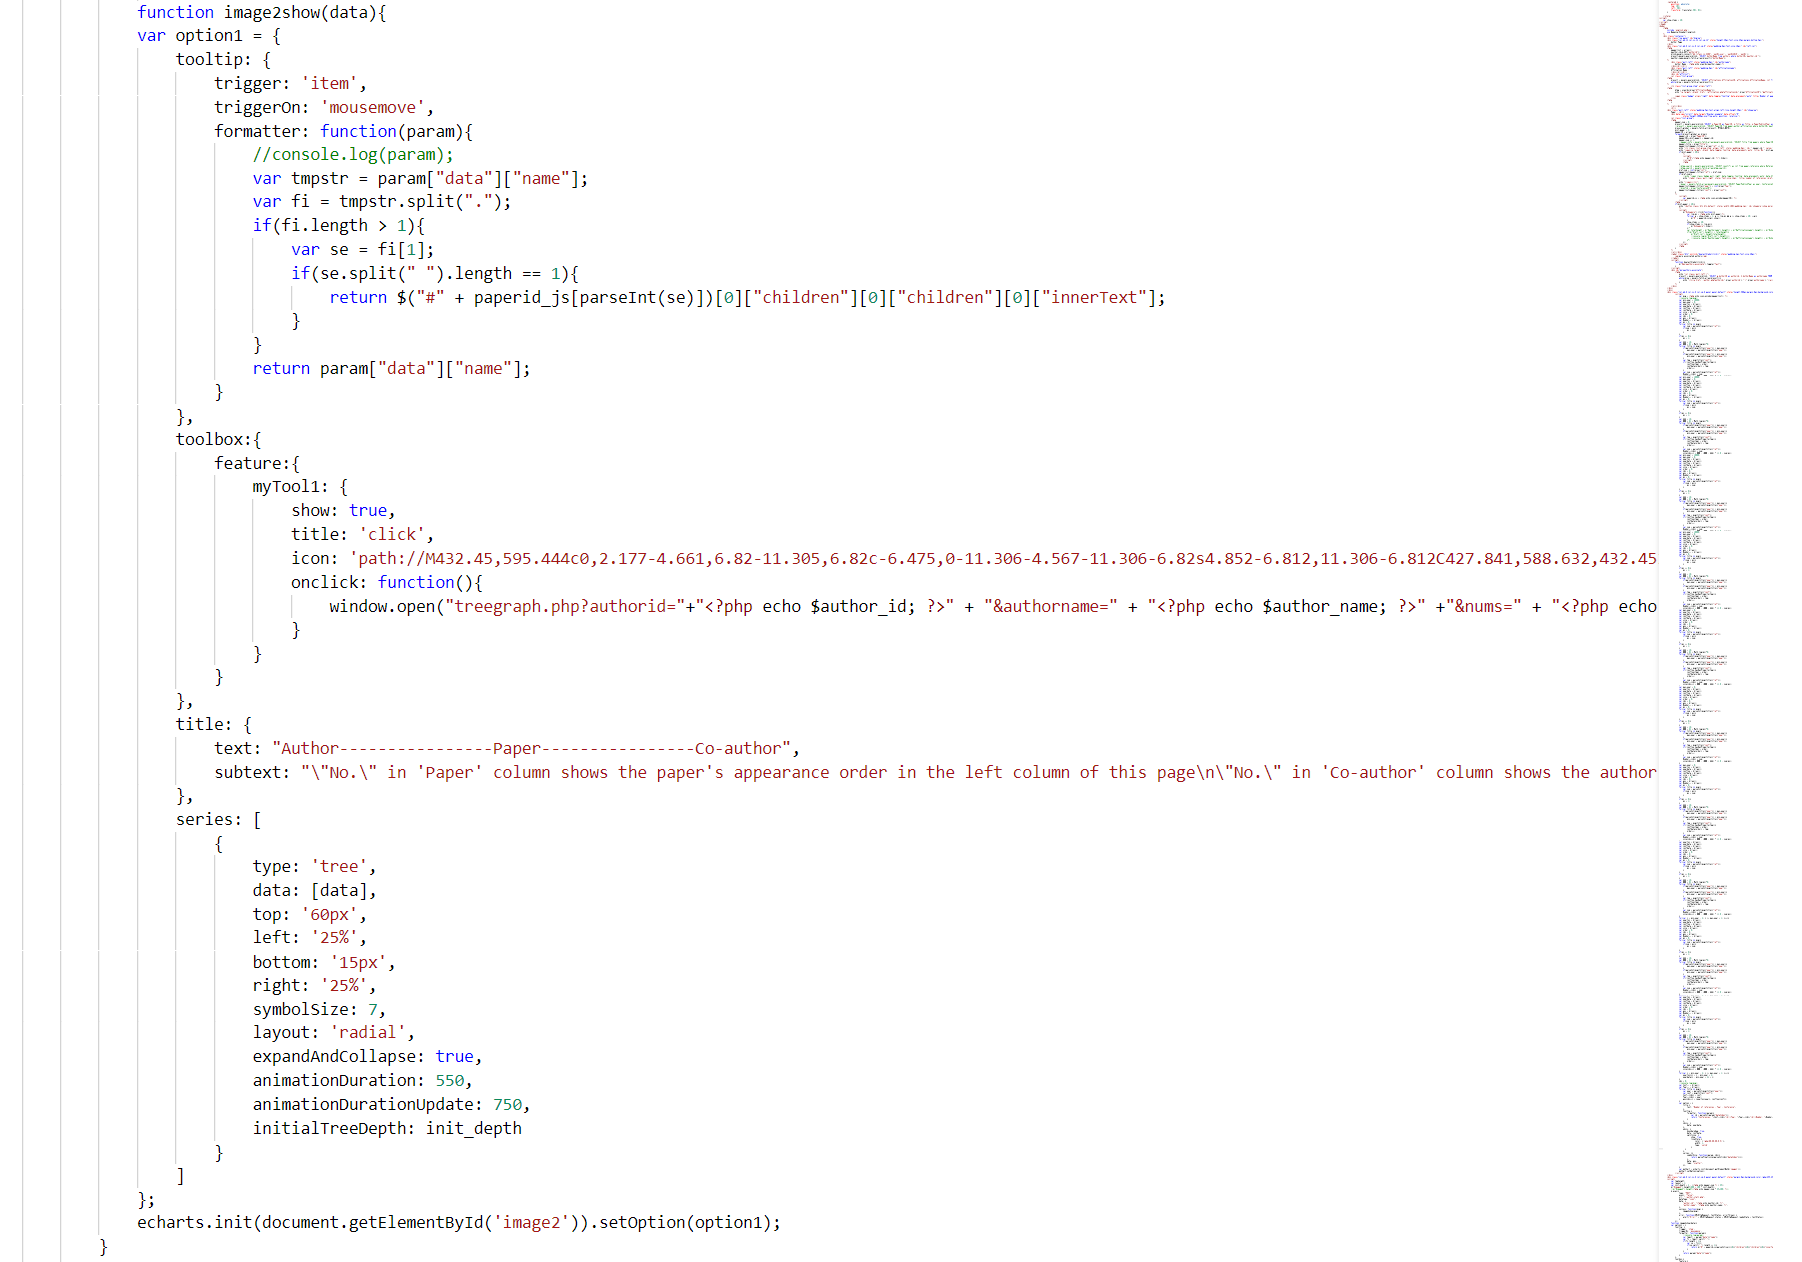
\includegraphics[width=0.5\textwidth]{treegraphcode2.png}
		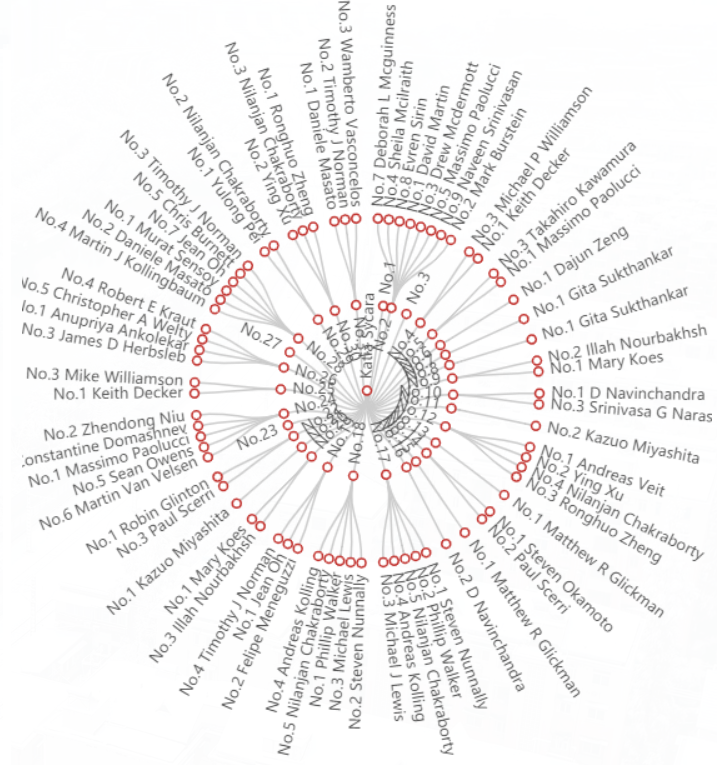
\includegraphics[width=0.5\textwidth]{treegraphimage.png}
	\end{figure}\
	\restoregeometry
	\newpage
	\section{Paper Page}
	The paper page can be visited through the link given in the \emph{Search Page} and \emph{Author Page} by pass the value of \emph{paper\underline{ }id} to \(Paper.php\). The \emph{Paper Page} consists of three parts : \emph{Basic Information Part}, \emph{Reference Part} and \emph{Citation Part}. The Page is built on \(bootstrap\), several \(div\) and \(rows\) are added into a \(div\) whose class is
	\(container\) to make the Page tidy and clear.
	\subsection{Basic Information Part}
	In this part, the basic information of the selected paper will be listed, including title, authors, published year and conference.
	\par To get all the required information, first, we use this command to get the \(ConferenceID\), \(title\) and \(publish year\) of the selected paper.
	\begin{figure}[H]
		\centering
		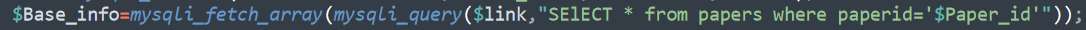
\includegraphics[width=0.9\linewidth]{p_1.png}
	\end{figure}
	Then we can get the conference name and all the authors of the paper with the following two \(SQL\) command and output them with a hyperlink by which can visit the corresponding \(Conference Page\) and \emph{Paper Page}.
	\begin{figure}[H]
		\centering
		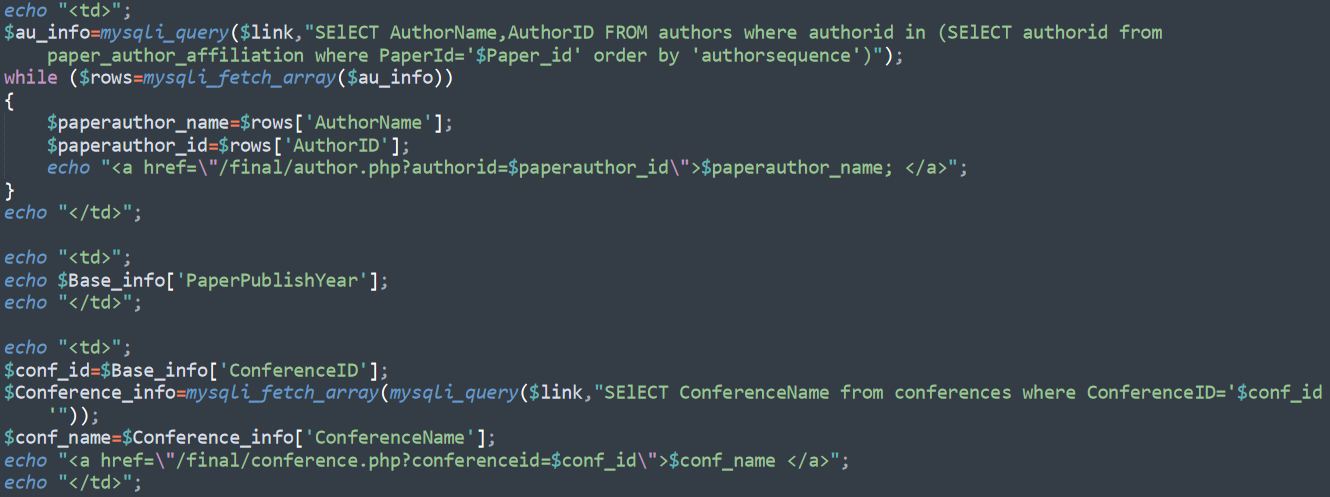
\includegraphics[width=0.9\linewidth]{p_2.png}
	\end{figure}
	And here is the basic information table.
	\begin{figure}[H]
		\centering
		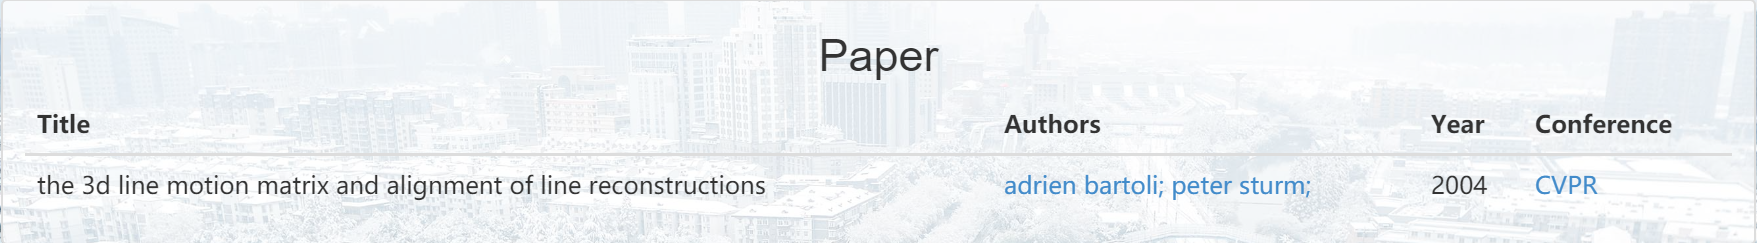
\includegraphics[width=1\linewidth]{bas_info.png}
		\caption{Basic Information}
	\end{figure}
	\subsection{Reference Part}
	The \emph{Reference Part} includes two parts. The first part is a table showing the detailed information of all the papers which were referred by the selected paper. And the second part is statistics of the reference information and their visualization.
	\subsubsection{Part I}
	In \(Part\ I\), considering that a paper can't refer to too many other papers, so we choose to list all the reference information in form of table. All the information is ordered by the publish year of the referred papers. In the table \(Conference\), \(Title\) and \(Author\) of the referred paper are given with links so that people can visit the corresponding page by clicking the link.
	\begin{figure}[H]
		\centering
		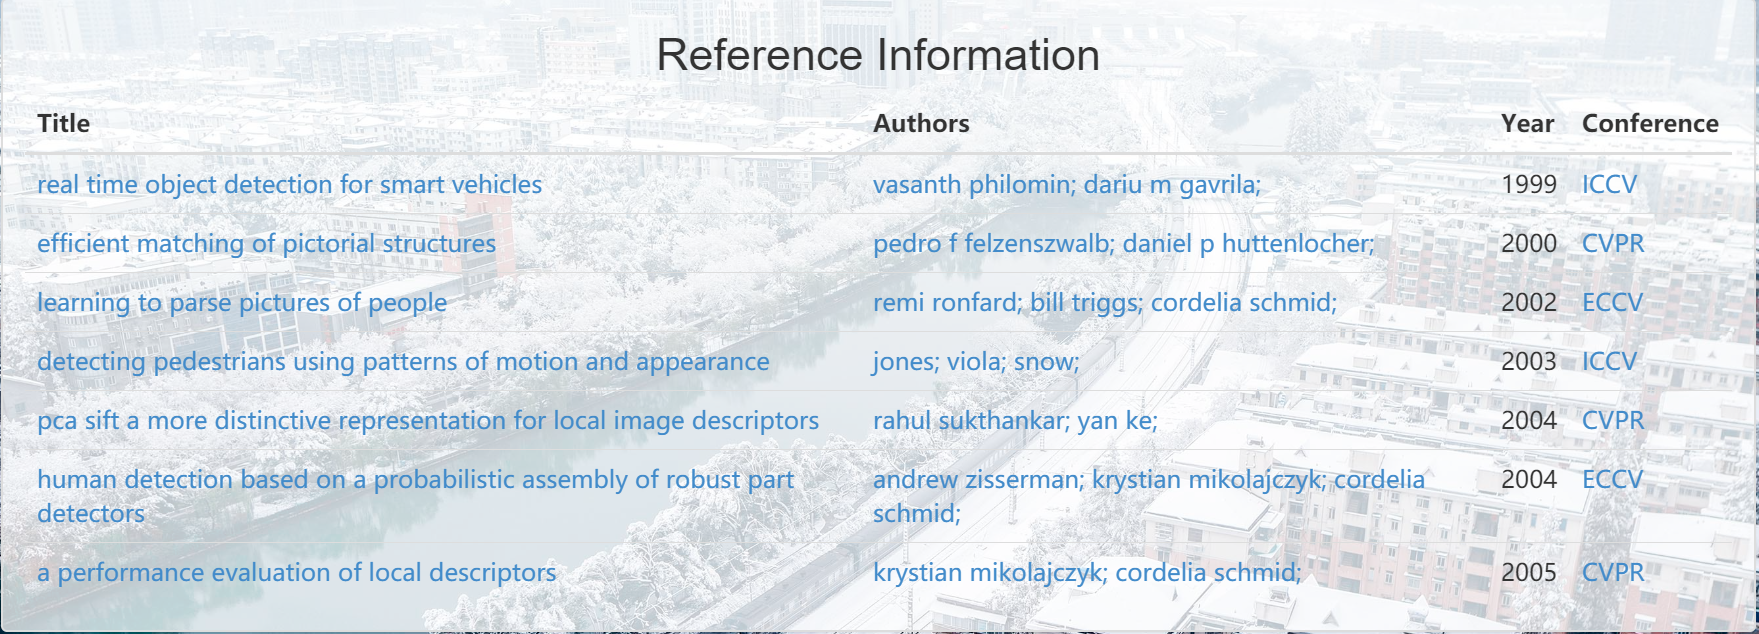
\includegraphics[width=0.9\linewidth]{p_3.png}
		\caption{Table of Information}
	\end{figure}
	\par The process of getting the required information is quite similar to the one in the \(Bacis Information Part\). First, we use the following command to get the \(PaperID\), \(ConferenceName\), \(ConferenceID\), \(Title\) and \(Publish Year\) of the referred papers.
	\begin{figure}[H]
		\centering
		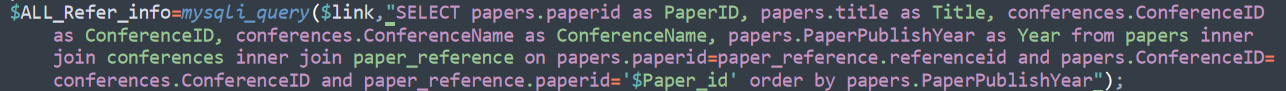
\includegraphics[width=0.9\linewidth]{p_8.png}
		\caption{get referred papers}
	\end{figure}
	\begin{figure}[H]
		\centering
		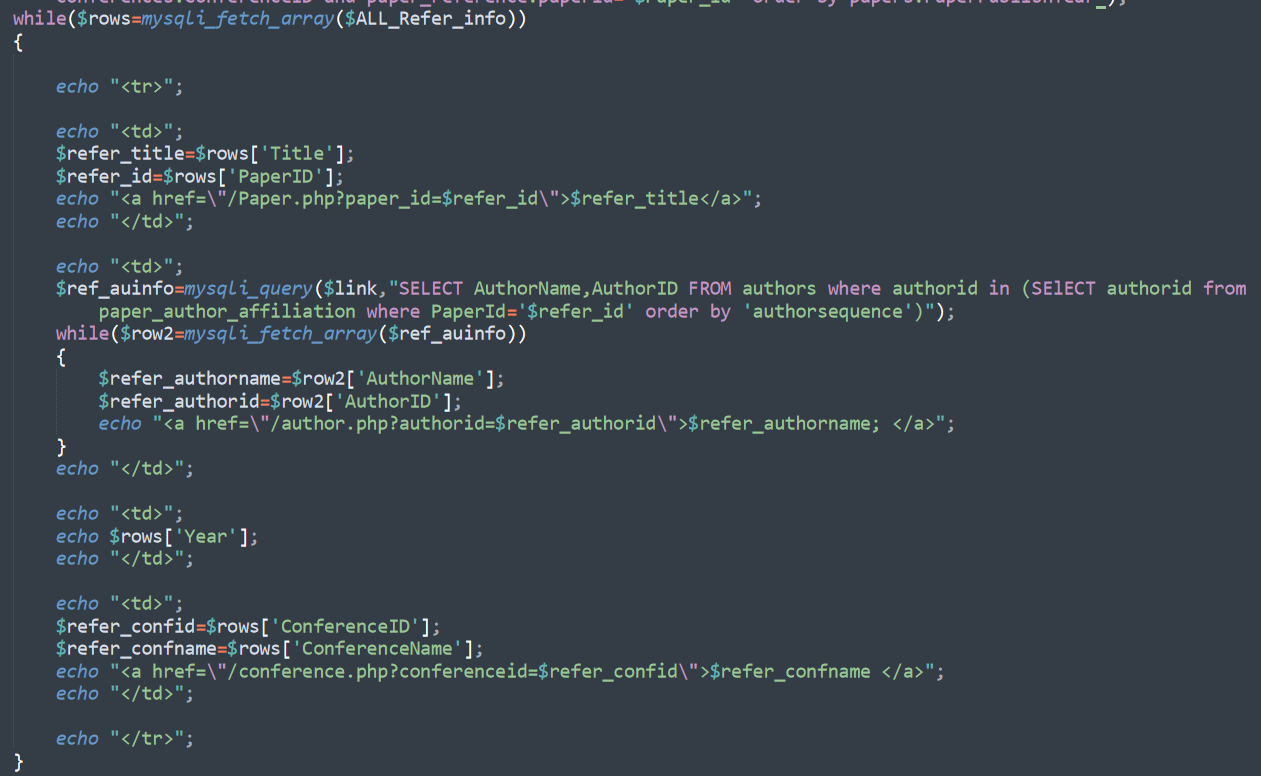
\includegraphics[width=0.65\linewidth]{p_9.png}
		\caption{output the result with hyperlink}
	\end{figure}
	Then Similarly, for each referred paper, we use another \(SQL\) command to get the authors from the table \(paper\)\underline{ }\(author\)\underline{ }\(affiliation\) and table \(authors\). Then we represent them in form of table with hyperlink which links to the corresponding pages.
	\subsubsection{Part II}
	In \(Part\ II\), three charts are given, including a pie chart, a histogram and a Reference tree, which represent the statistics of different data.
	\\
	\\
	\textbf{Pie\ Chart}
	\par The first part shows the distribution of the papers in different conferences. Put the mouse on the figure and it will show the detailed number.
	\begin{figure}[H]
		\centering
		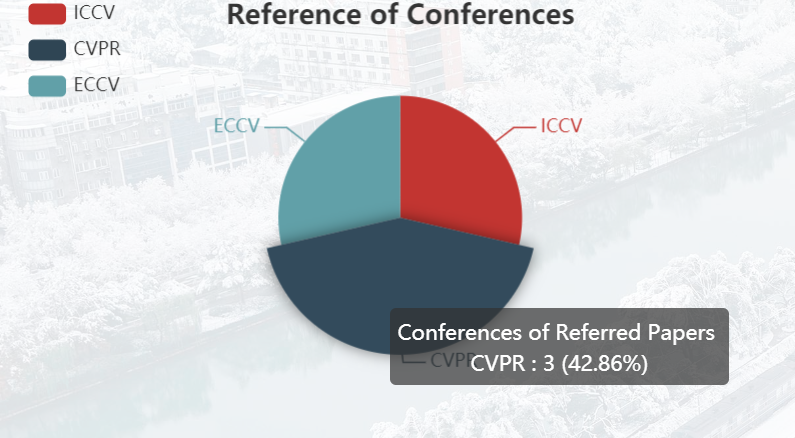
\includegraphics[width=0.5\linewidth]{p_4.png}
		\caption{Pie figure}
	\end{figure}
	To get the required Information, we use \(ajax\) to connect another \(php\) and post the necessary parameter to it. And the \(ajax\) will run the function \emph{refer\underline{ }bing\underline{ }show()}, which use \(Echarts\) to visualize the data in form of pie chart.
	\begin{figure}[H]
		\centering
		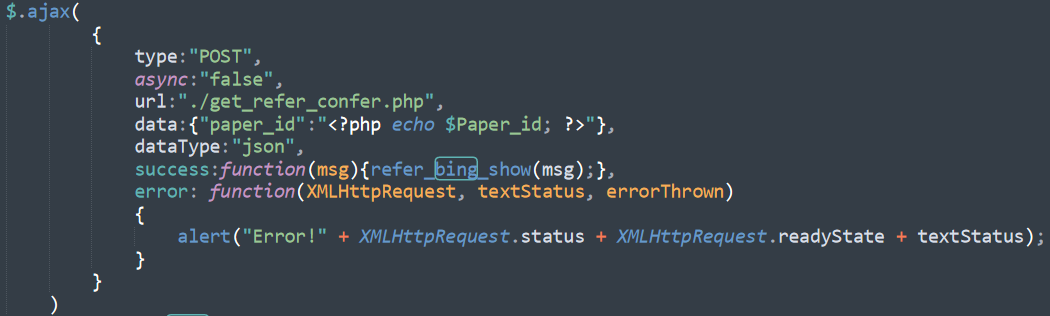
\includegraphics[width=0.7\linewidth]{p_10.png}
	\end{figure}
	In \emph{get\underline{ }refer\underline{ }confer.php}, we use following \(SQL\) commands to get the names of the conferences and the referred papers. Then we make a simple calculation of the distribution of papers in different conference. Then we return the result in \(json\) form.
	\begin{figure}[H]
		\centering
		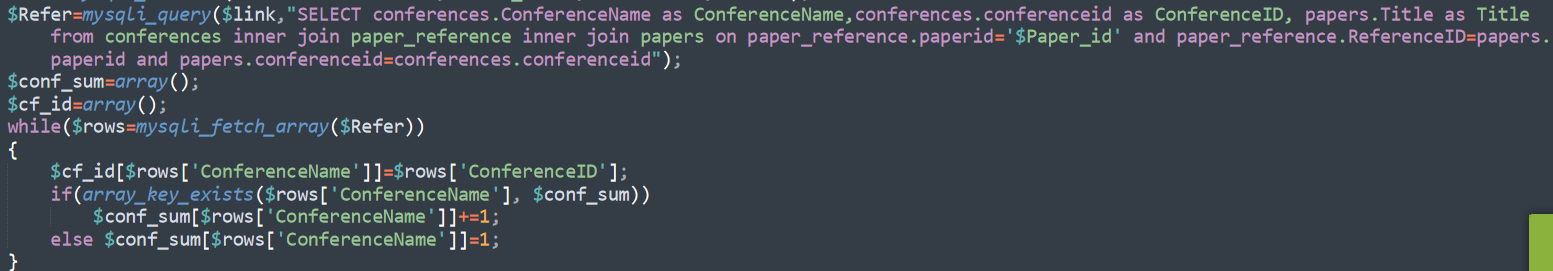
\includegraphics[width=0.9\linewidth]{p_11.png}
		\caption{\(SQL\) commands}
	\end{figure}
	\begin{figure}[H]
		\centering
		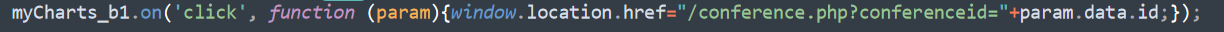
\includegraphics[width=0.9\linewidth]{p_12.png}
		\caption{function \(on()\)}
	\end{figure}
	Also, the function \(on()\) of \(Echarts\) is redefined, which adds a hyperlink to the corresponding part in the chart so that people can visit \(Conference Page\) by clicking the sector.
	\\
	\\
	\\
	\textbf{Histogram}
	\par The second figure shows how many papers are referred in different years. Put the mouse on the figure and we can see the detailed information. The selected part is highlighted.
	\begin{figure}[H]
		\centering
		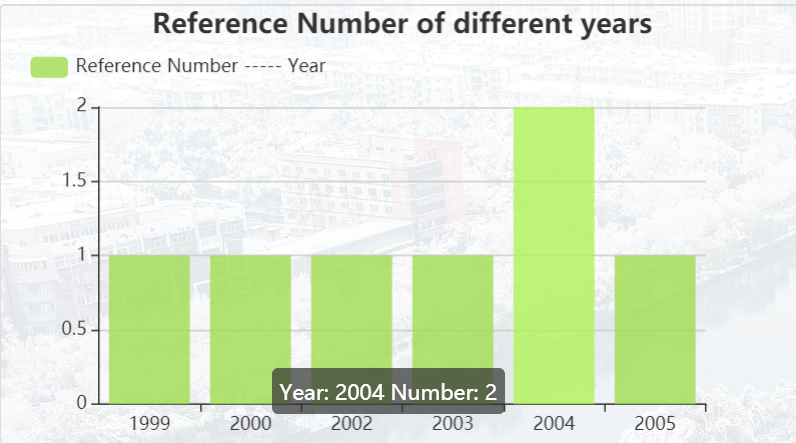
\includegraphics[width=0.6\linewidth]{p_5.png}
	\end{figure}
	Similarly, we use the \(ajax\) to get necessary information.And in \emph{get\underline{ }refer\underline{ }year.php}, we use this \(SQL\) command to get all the referred papers' publish year and use several loop statements to make a statics. Then we return the result to \(ajax\) in form of \(json\).
	\begin{figure}[H]
		\centering
		
		\subfigure[\(ajax\)]{
			\begin{minipage}[h]{0.6\linewidth}
				\centering
				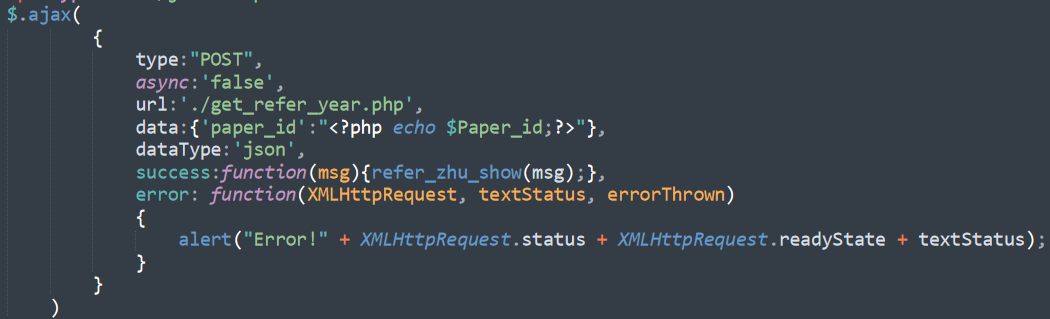
\includegraphics[width=0.95\linewidth]{p_13.png}
				%
			\end{minipage}%
		}%
		\subfigure[Statics]{
			\begin{minipage}[h]{0.4\linewidth}
				\centering
				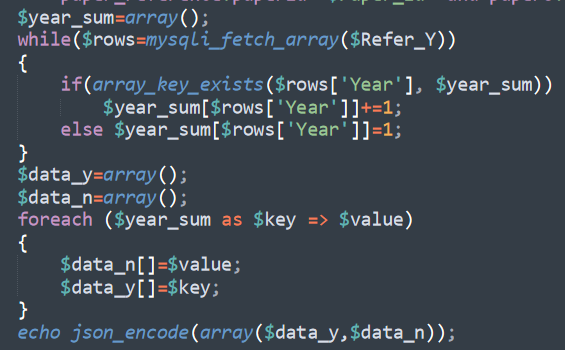
\includegraphics[width=0.9\linewidth]{p_15.png}
				%
			\end{minipage}%
		}%
	\end{figure}
	\begin{figure}[H]
		\centering
		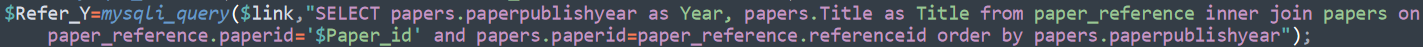
\includegraphics[width=1\linewidth]{p_14.png}
		\caption{\(SQL\) command}
	\end{figure}
	Also, we the \(toolip\) in the option of \(Echarts\) is redesigned as follows:
	\begin{figure}[H]
		\centering
		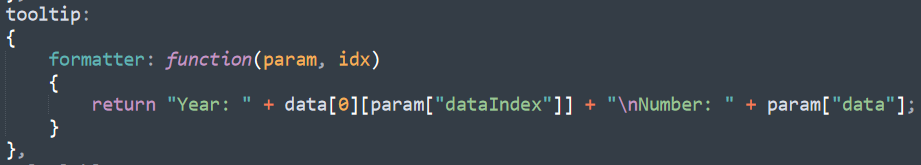
\includegraphics[width=0.7\linewidth]{p_16.png}
	\end{figure}
	Then once we put our mouse on the chart, we can see the detailed number of each year.
	\\
	\\
	\textbf{Reference\ Tree}
	\par The third part is the reference tree, which shows the reference relations clearly. The process of getting data is quite similar with the previous two. A \(ajax\)  is also used in this part. In \emph{get\underline{ }refer.php}, we select the titles and the conferences' names of the referred papers by this \(SQL\) command. Then we sort then by their conferences' names and gather then in the layout of a tree.
	\begin{figure}[H]
		\centering
		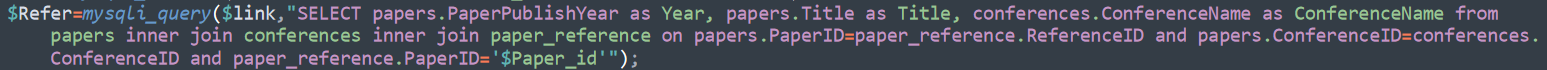
\includegraphics[width=0.9\linewidth]{p_17.png}
		\caption{\(SQL\) command}
	\end{figure}
	\begin{figure}[H]
		\centering
		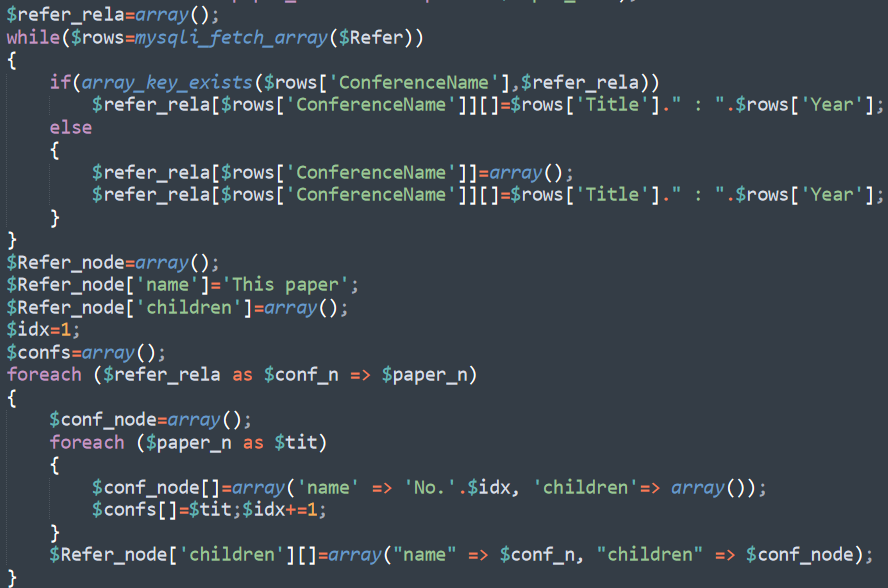
\includegraphics[width=0.6\linewidth]{p_18.png}
		\caption{Sorting}
	\end{figure}
	The titles of the papers are very long, which means it's really inconvenient to print them on the screen directly. So we redesigned the \(toolip\) in the option of the chart. We use \(No.\) with number to represent the papers on the reference tree and The number of each paper is given randomly. When the visitors of the Page put their mouse on the node of papers, the detailed information of paper, including title and the publish year of papers will be shown.
	\begin{figure}[H]
		\centering
		
		\subfigure[\(toolip\)]{
			\begin{minipage}[h]{0.45\linewidth}
				\centering
				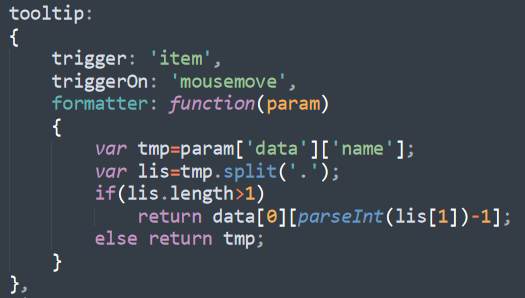
\includegraphics[width=0.9\linewidth]{p_19.png}
				%
			\end{minipage}%
		}%
		\subfigure[Reference Tree]{
			\begin{minipage}[h]{0.55\linewidth}
				\centering
				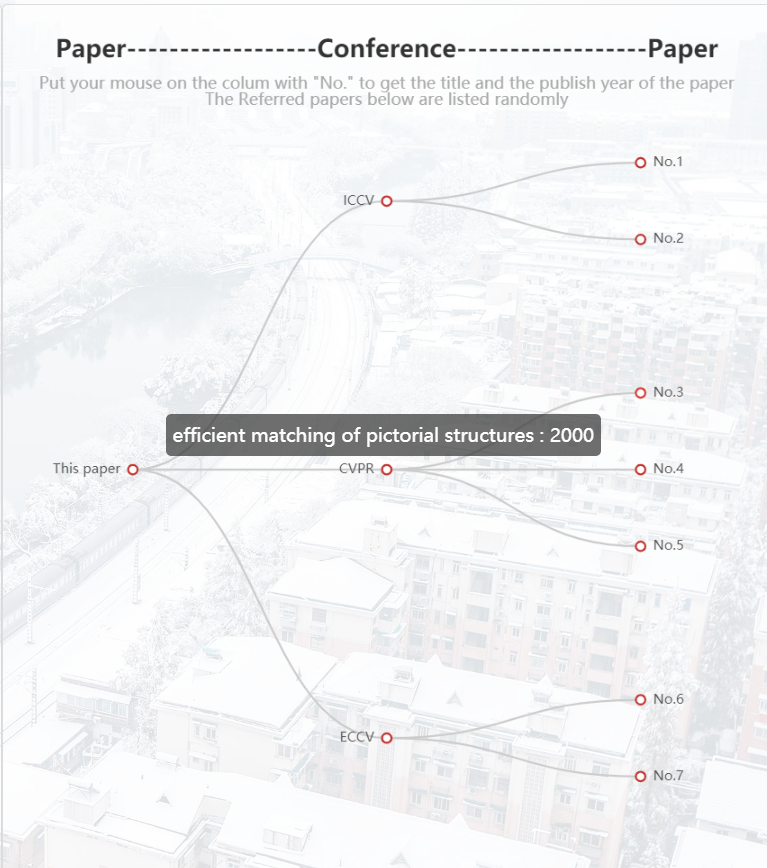
\includegraphics[width=0.8\linewidth]{p_7.png}
				%
			\end{minipage}%
		}%
	\end{figure}
	\par And because the height of the tree is not fixed so the height of this \(div\) in \(html\) is also flexible. The height of this \(div\) has the relation below.
	\begin{figure}[H]
		\centering
		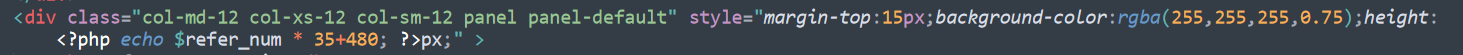
\includegraphics[width=1\linewidth]{p_6.png}
		\caption{Relation}
	\end{figure}
	The more papers are referred, the larger the \(div\) is so that the charts will not be out of range.
	\subsection{Citation Part}
	The \(Citation\ Part\) also includes two part. The first part is the citation information in form of tables. And the second part is statistics of the citation information and their visualization. The structure of \(Citation\ Part\) is quite similar with the \(Reference\ Part\) so we will not show the repeated or similar codes in this part of report. What we will do is to show the different part and the additional function.
	\subsubsection{Part I}
	In \(Part\ I\), we just list the newest 15 (at most) citation records in the table, because a paper might be referred by many papers for many times and if we list all information the size of the table will be extremely huge, which makes the Page ugly. The process of getting data and output is similar with the one in \(Reference\ Part\), and just some slight code adjustment can make it. In this part you can see the \(Titles\), \(Authors\), \(Published\ Years\) and \(Conferences\) of each paper. And to get all the detailed information by clicking the hyperlink.
	\begin{figure}[H]
		\centering
		\includegraphics[width=0.6\linewidth]{P_20.png}
		\caption{The hyperlink to the \(Detailed\ Information\ Page\)}
	\end{figure}
	The hyperlink given in the figure above gives visitors a way to visit the \(detailed\ information\ page\).
	\\
	\\
	\textbf{Detailed Information Page}
	\par The \(Detailed\ Information\ Page\) will list all the detailed citation information in form of tables, including \(Titles\), \(Authors\), \(Published\ Years\) and \(Conferences\). Considering the size of the page and the data, only 15 lines of information will be listed in one page and the turning page function is designed.
	\begin{figure}[H]
		\centering
		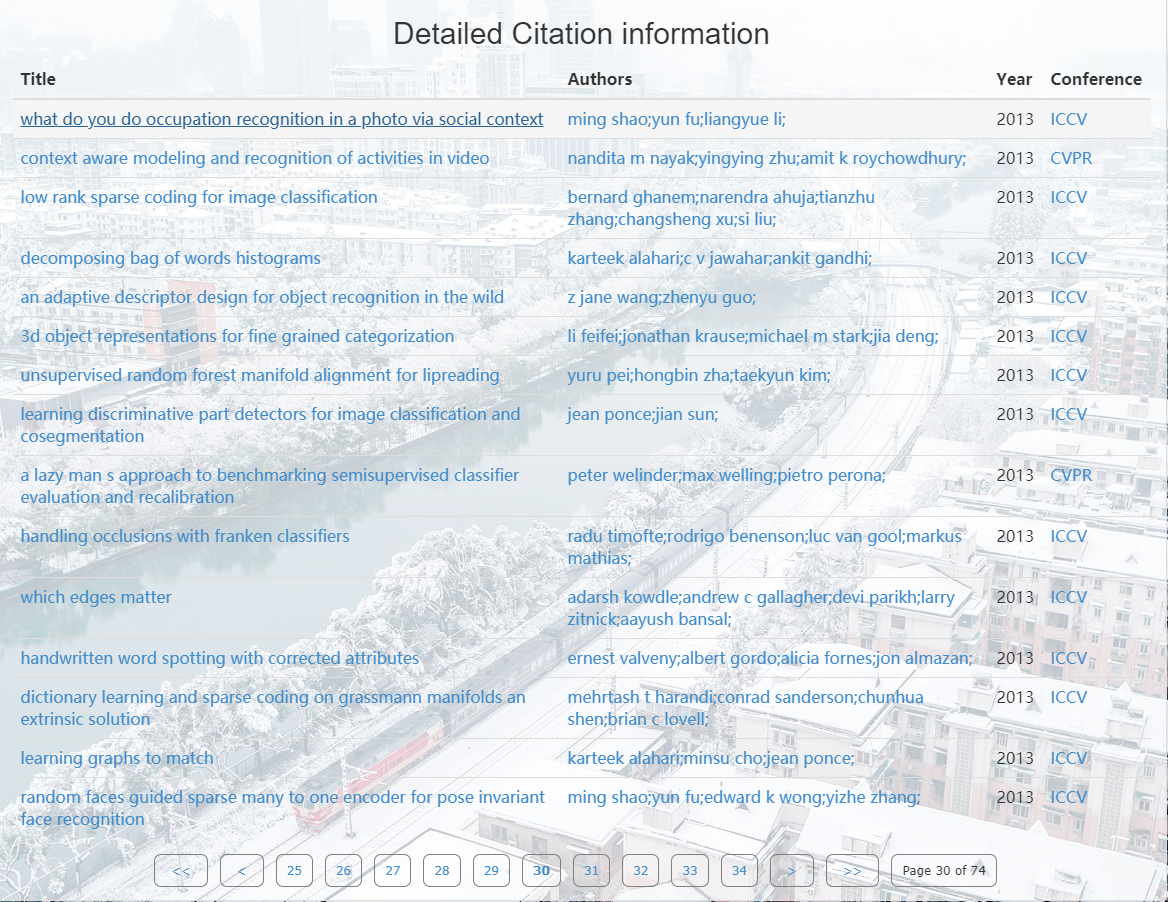
\includegraphics[width=0.7\linewidth]{p_21.png}
		\caption{Detailed Information Page}
	\end{figure}
	The information in every page is different depending page number, which gives a limited range to the result. So we can't use fixed commands to get necessary information. To do this we must use \(function\) in our \(php\) commands.
	\par First, we need to get the \emph{Paper\underline{ }id} and the \(Page Number\) of the current page. They will be posted by the hyperlink. And other basic variables to limit the range are also initialized at the beginning of the program. The @ in the code means ignore the potential warning so that the code can run fluently.
	\begin{figure}[H]
		\centering
		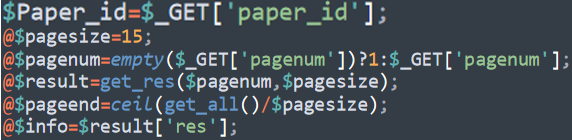
\includegraphics[width=0.6\linewidth]{p_22.png}
		\caption{Initialization}
	\end{figure}
	\begin{figure}[H]
		\centering
		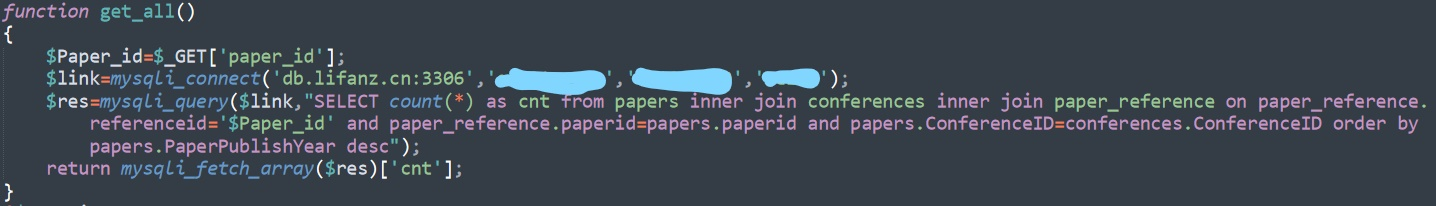
\includegraphics[width=0.9\linewidth]{p_23.jpg}
		\caption{\(get\)\underline{ }\(all()\) function}
	\end{figure}
	The \(get\)\underline{ }\(all()\) use \(SQL\) commands like \(SELECT\) and \(count(*)\) to get the size of data and return it as the result. With the size of the data, we calculate the total pages of the detailed information.
	\par The data to be represent is not fixed depending on the page number. To collect the data, we need another function.
	\begin{figure}[H]
		\centering
		\includegraphics[width=0.7\linewidth]{P_24.jpg}
		\caption{\(get\)\underline{ }\(res\)() function}
	\end{figure}
	The \(get\)\underline{ }\(res\)() function use \(SELECT\) command with parameter \(limit\) to get the data to be represented. In \(SQL\) commands, \(Limit\) is used in form of \{\(Limit\ a,b\)\}, which means this \(SQL\) will select from the \(No.a\) result to the \(No.(a+b-1)\) result and return them as the final result of the query (The number of the results starts from 0, which means \(a\ge 0\)). The result of the \(SQl\) query includes \(PaperID\), \(ConferenceID\), \(Title\), \(ConferenceName\) and \(Published Year\). The \(PaperID\) and \(ConferenceID\) is used for adding hyperlink. And to get the authors of the papers, we use another \(SQL\) command in the loop the get information from the table \(Authors\) and \emph{paper\underline{ }author\underline{ }affiliation}. Then we merge them all together and return it as the result of the function \(get\)\underline{ }\(res\)(). The output process is almost the same as the one in \(Part\ I\) of \(Reference\ Part\). Only some small adjustment in codes can make it, so we will not do any more introduction about it.
	\par At the end of this page is the buttons for turning pages. Every button has hyperlink goes to the corresponding page. The button with \(<\) and \(>\) goes to the previous and next one page, the button with \(<<\) and \(>>\) goes to the first and the last page. Also ten buttons is listed, which goes to the 10 pages nearby the current page. The text on the button of the current page is emphasized.
	\begin{figure}[H]
		\centering
		
\includegraphics[width=0.9\linewidth]{p_25.png}
		\caption{buttons}
	\end{figure}
	The style of the buttons is redesigned with \(CSS\).
	\begin{figure}[H]
		\centering
		
		\subfigure[\(CSS\)]{
			\begin{minipage}[h]{0.3\linewidth}
				\centering
				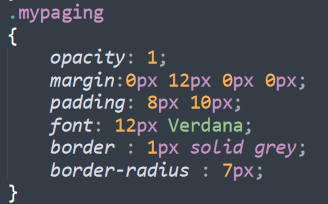
\includegraphics[width=0.9\linewidth]{p_26.png}
				%
			\end{minipage}%
		}%
		\subfigure[Codes of buttons]{
			\begin{minipage}[h]{0.7\linewidth}
				\centering
				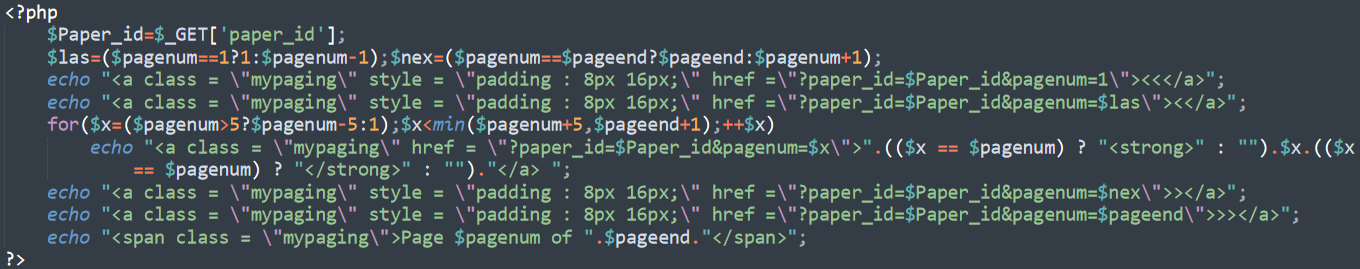
\includegraphics[width=0.95\linewidth]{p_27.png}
				%
			\end{minipage}%
		}%
	\end{figure}
	\subsubsection{Part II}
	The Second Part of \(Citation\ Part\) also consists of three parts:  a pie chart, a histogram and a Citation tree, which represents the statics of the data.
	\\
	\\
	\textbf{Pie Chart}
	\par The pie chart shows the distribution of the papers in different conferences. The process of getting necessary information is almost the same as the one in the \(Reference\ Part\). Just some small adjustment of codes can make it. I want to show that the number of the conferences may be large and the proportion of the papers in different conferences might be not so balanced so some sector on the pie chart might be difficult to be seen. In this situation, visitors can click the legends on the left of the chart then the chart will hide the corresponding sector and the legend will turn grey. if visitors want to see the hidden sectors, just click the legend again.
	\begin{figure}[H]
		\centering
		
		\subfigure[]{
			\begin{minipage}[h]{0.5\linewidth}
				\centering
				\includegraphics[width=0.9\linewidth]{p_29.png}
				%
			\end{minipage}%
		}%
		\subfigure[]{
			\begin{minipage}[h]{0.5\linewidth}
				\centering
				\includegraphics[width=0.9\linewidth]{p_30.png}
				%
			\end{minipage}%
		}%
	\end{figure}
	This will make it more convenient to click or read the detailed data.
	\\
	\\
	\textbf{Histogram}
	\par The histogram in \(Citation\ Part\) is a little bit different this time we count the citation in different year and different conferences. Put the mouse on the histogram, the year and the exact number of the selected part will be shown. To get the necessary information, we use \(ajax\) to post the \(Paper\)\underline{ }\(id\) to a \(php\) and use \(SQL\) command to get the conferences' names and publish years of every citation. We find that the distribution of papers might be dispersive, which makes the chart difficult to be seen clearly. so a \(datazoom\) is added into the option of the chart.
	\begin{figure}[H]
		\centering
		
		\subfigure[\(datazoom\)]{
			\begin{minipage}[h]{0.4\linewidth}
				\centering
				\includegraphics[width=0.7\linewidth]{p_28.png}
				%
			\end{minipage}%
		}%
		\subfigure[]{
			\begin{minipage}[h]{0.6\linewidth}
				\centering
				\includegraphics[width=0.7\linewidth]{p_31.png}
				%
			\end{minipage}%
		}%
	\end{figure}
	
	\begin{figure}[H]
		\centering
		
		\subfigure[]{
			\begin{minipage}[h]{0.5\linewidth}
				\centering
				\includegraphics[width=0.8\linewidth]{p_32.png}
				%
			\end{minipage}%
		}%
		\subfigure[]{
			\begin{minipage}[h]{0.5\linewidth}
				\centering
				\includegraphics[width=0.8\linewidth]{p_33.png}
				%
			\end{minipage}%
		}%
	\end{figure}
	\(Datazoom\) give the chart two sliders. visitors can control the size of the chart by the sliders, also they can control it by the mouse wheel. Once the visitors wants to see the part of the whole chart, they can enlarge the chart. But we need to emphasize that the mouse wheel can only control the zooming of the x-axis.
	\\
	\\
	\textbf{Citation Tree}
	\par The citation tree shows the citation relations directly, But we know that the citation tree might be very big, which makes the page impossible to be seen clearly. So we adjust the type of the tree depending on the size of data. When there are more than thirty lines of citation information the tree will be displayed by radial type. To make it, we change the \(layout\) of \(series\) in the option of the chart into \(radial\).
	\begin{figure}[H]
		\centering
		\includegraphics[width=0.25\linewidth]{P_37.png}
	\end{figure}
	\begin{figure}[H]
		\centering
		
		\subfigure[less than 30]{
			\begin{minipage}[h]{0.33\linewidth}
				\centering
				\includegraphics[width=0.8\linewidth]{p_34.png}
				%
			\end{minipage}%
		}%
		\subfigure[greater than 30(depth=2)]{
			\begin{minipage}[h]{0.33\linewidth}
				\centering
				\includegraphics[width=0.8\linewidth]{p_35.png}
				%
			\end{minipage}%
		}%
		\subfigure[greater than 30(depth=3)]{
			\begin{minipage}[h]{0.33\linewidth}
				\centering
				\includegraphics[width=0.8\linewidth]{p_36.png}
				%
			\end{minipage}%
		}%
	\end{figure}
	And to avoid the situation that too many papers are represents at the same time, the initial depth of the radial tree is set as 2. The visitors can expand the tree by clicking the nodes on the tree.
	\par For the situation that we need to use radial tree, we design another page for visitors to see the whole tree in normal way. Click The symbol of eye then the visitors can go to the page of big citation tree.
	\begin{figure}[H]
		\centering
		\includegraphics[width=0.75\linewidth]{P_38.png}
	\end{figure}
	To realize the function, we design one tool in the toolbox of the chart. The eye is drawn by \(Path\) which use coordinate and other parameter to represent lines and points.
	\begin{figure}[H]
		\centering
		\includegraphics[width=0.8\linewidth]{P_39.png}
	\end{figure}
	The realization of the Big citation tree page is not the same as the small citation tree or reference tree. Put the mouse on the tree ,the title and the publish year will be shown too. We have to emphasize that the tree is large so the visitors might have to wait for a minute before the tree can be seen.
	\newgeometry{left=2.3cm,right=2.3cm,top=2cm,bottom=2cm}
	\section{About Conference Page}
	The conference page presents the information and basic condition of one specific conference.\\
	Click any name of conference in other pages to see its ocnference page.\\
	I will introduce this page as separated parts.
	\subsection{Title}
	\includegraphics[width=\textwidth]{title1.png}\\
	\centerline{\small The Confernce Name}
	Here I use abbreviation for the conference name so that when focusing on it we can see its full name.
	
	\subsection{List of Authors}
	In this part I list the authors in two ways, and it can be switched by the buttons above:
	\begin{itemize}
		\item Here I rank the ten best authors according to the scores assigned by my teammate.\\\\\includegraphics[width=0.9\textwidth]{author1.jpg} \\
		\item Here I list all the authors by the number of papers.\\\\\includegraphics[width=0.9\textwidth]{author2.jpg}\\
		\item The source code:\\\includegraphics[width=\textwidth]{authorcode1.jpg}\\
	\end{itemize}
	
	\large When collecting the infomation, I use a lot MySQL inquiring statements. And they are used in most of other parts. So I show them {\bfseries together} here:\\
	\includegraphics[width=\textwidth]{code0.png}
	\subsection{List of Papers}
	This part is similar to the former part. I list the best authors according to their times of being referred to. And by clicking buttons, it can show all the authors order by the first letter.\\\\
	\includegraphics[width=0.5\textwidth]{author3.jpg}
	\includegraphics[width=0.5\textwidth]{author4.jpg}\\\\
	The second one has the categorizing fucntion. \\
	The basic idea is to assign IDs to each term corresponding to their first letter, and when categorized, it just need to hide others.\\
	And this way is also used to the tab buttons.\\\\
	\includegraphics[width=0.5\textwidth]{tab1.png}
	\includegraphics[width=0.5\textwidth]{tab.png}\\
	
	\subsection{Word Cloud for Titles}
	This word cloud is generated statically on the website "wordart.com".\\\\
	\includegraphics[width=\textwidth]{wc.jpg}\\\\
	And each term in this cloud has a hyperlink to its search result page.\\
	
	\subsection{Chart for Article Counts}
	This chart is realized by the Echarts API. Actually I do not need to set anything but the data by myself.\\
	This histogram (or line graph when switched) is to present the number of papers for each year.\\
	The tools are supported by Echarts.\\\\
	The functions are as follows:\\
	\includegraphics[width=0.5\textwidth]{year.jpg}
	\includegraphics[width=0.5\textwidth]{year1.jpg}
	
	\subsection{Graph for Authors}
	The final part which is located in the bottom of the page is about the reference realtions between the authors.\\\\
	Altogether there are thousands of authors and hundreds of thousands of relationships in one conference.\\
	However, most of the authors have only arbitrary relationships with others, which is of little value for us.\\\\
	So I only take 100 authors to draw this graph. Also it's almost the maximum because of the calculation performance of the browser.\\\\
	\newpage
	The setting for points:\\
	\includegraphics[width=\textwidth]{code3.jpg}\\
	The setting for lines:\\
	\includegraphics[width=\textwidth]{code4.jpg}\\\\
	The graph has two styles --- circular layout or force orientation.\\\\
	\includegraphics[width=\textwidth]{circular.jpg}\\\\
	\includegraphics[width=\textwidth]{force.jpg}\\
	\restoregeometry
\end{document}
	 
